\chapter{Estudio de Canales de Comunicación de Hardware}
La segunda hipótesis para explicar la mala performance del caso de estudio presentado se centra en una arista relacionada hardware más que al software mismo. Cómo ya se mencionó, la capacidad multiprocesador de que se dispone en equipos modernos no es un recurso fácil de aprovechar, de hecho, se requiere de una sofisticada operación y diseño tanto de las aplicaciones que solicitan recursos como del sistema operativo que ha de administrarlos, para conseguir las anheladas mejoras de performance. Como se repasó en secciones anteriores, la capacidad de paralelismo viene dada gracias a un conjunto de protocolos y algoritmos de muy bajo nivel que coordinan y mantienen en estado coherente las distintas componentes de datos para los diferentes procesadores disponibles en un esquema \emph{SMP} \cite{paper:MESI, paper:snoop}, sin embargo, por muy sofisticados que dichos mecanismos sean, las nuevas tecnologías de hardware que prometen velocidades de trasferencia y acceso nunca antes imaginadas podrían significar un problema para dichas componentes, sobrepasándolas de cierta forma.

Es precisamente en ésta línea que se establece la segunda hipótesis. En éste caso, se adjudican las responsabilidades por el mal rendimiento presentado en el caso de estudio a un problema de contención de recursos (nuevamente relacionado al spinlock de los Internet sockets), pero ésta vez, asociado a la persistencia y disponibilidad que se da del mismo a través de los mecanismos de coordinación antes mencionados. En las arquitecturas modernas los protocolos \emph{MESI} y de \emph{SNOOP} son cruciales en la operación de ejecuciones paralelas para garantizar integridad en los datos, pero las arquitecturas modernas proponen nuevas distribuciones de los componentes internos de hardware, brindando canales de comunicación de mayor velocidad de transmisión y reasignando los recursos físicos en modos diferentes a los usados para la concepción de los mecanismos de control ya mencionados. Ésta hipótesis plantea la posibilidad de que el defecto de performance del caso de estudio sea generado por un fenómeno de \emph{Caché Bouncing}, producto del abusivo comportamiento de dichos mecanismos de control en las arquitecturas modernas.

\begin{defn}[ver \cite{paper:cachebouncing}] \textbf{Caché Bouncing} corresponde a un fenómeno producido en entornos multiprocesador, cuando distintas CPU realizan modificaciones a una línea de caché especifica que está siendo referenciada por varios procesadores. La modificación de la línea en cuestión se propaga de caché en caché según los protocolos de consistencia del sistema, pero cuando la cardinalidad de referencias de los distintos procesadores sobre la misma línea de caché es muy alta, los mecanismos de propagación de caché pueden operar deficientemente. Éste fenómeno impone una significativa carga en el bus de memoria y los distintos canales de comunicación afectados pudiendo degenerar desde una degradación del proceso responsable hasta una degradación generalizada de la performance del sistema.
\end{defn}

En ésta línea, el fenómeno de \emph{Cache Bouncing} se podría manifestar dada la arquitectura del sistema, la que al contemplar bancos de memoria diversos --algunos compartidos y otros exclusivos para los núcleos de procesamiento-- podría estar manifestándose como resultado de las modificaciones concurrentes de los distintos procesadores sobre la estructura socket compartida, y más precisamente sobre el spinlock de protección del socket. Lo anterior combinado a la operación de los protocolos de consistencia y correctitud para las líneas de caché del sistema postulan evidencia que hace perfectamente posible el diagnóstico de que se esté generando un escenario de sobrecarga de comunicación que termine degradando los tiempos totales de ejecución del caso de estudio.

Para validar la hipótesis anterior es preciso un cabal entendimiento de la arquitectura de hardware objetivo a fin de poder localizar puntos de contención y canales afectados. Junto con lo anterior, se hace crucial una comprensión significativa del funcionamiento de la \emph{Performance Monitoring Unit} que provee el fabricante, así como lograr configurarla y aprovecharla para la recolección de datos finales. En las siguientes secciones se realiza un estudio de la arquitectura descrita en la figura \ref{fig:pc3} del equipo sobre el cual se realizan las pruebas experimentales reales para poder acotar el dominio de estudio. Posteriormente se realiza un análisis experimental de las tendencias presentes en una tarea de acceso concurrente como la descrita en el caso de estudio de ésta investigación con el fin de corroborar o descartar las sospechas ya mencionadas del efecto de contención y \emph{caché bouncing} por eventos de performance de hardware.

\section{Características de Arquitecturas de Hardware Modernas}
Cómo ya se mencionó en secciones anteriores, los fabricantes de partes y piezas de computadoras están constantemente desarrollando importantes avances, de la mano con el desarrollo técnico de piezas que brinda mejores componentes de hardware cada día, y la línea de desarrollo de infraestructura de hardware principal de los computadores no está exenta de dicha evolución. En secciones anteriores se presentó como las arquitecturas han evolucionado desde el primer esquema \emph{SMP} propuesto con la distribución \emph{FSB}, pasando luego por nuevas configuraciones como \emph{DIB} y \emph{DHSI}, entre otras. Sin embargo, el desarrollo ha sido constante y hoy las arquitecturas han degenerado en esquemas bastante más complejos en pos de aprovechar al máximo la capacidad de los procesadores en la línea del paralelismo.

\subsection{Arquitectura Intel QuickPath}
El año 2008, el fabricante de procesadores Intel®\footnote{\url{http://www.intel.com/}} lanzó al mercado una nueva tecnología denominada \emph{Intel QuickPath Architecture} \cite{paper:quickpath} la que postuló un nuevo esquema organizacional de los componentes internos de la placa principal de las computadoras, así como también un nuevo esquema de conectividad entre los componentes de la misma, prometiendo entre otras cosas, un sistema más confiable, eficiente, rápido y escalable, que podría aprovechar mejor la capacidad de los múltiples procesadores de su misma línea. Rápidamente \emph{QuickPath} se posicionó en el mercado para competir con la tecnología \emph{HyperTransport} desarrollada por \emph{AMD}\footnote{Principal competidor de Intel en la industria de la manufactura de microprocesadores.}, abriendo paso definitivamente a una era, dejando atrás el enfoque \emph{FSB}.

\begin{figure}[!h]
	\centering
	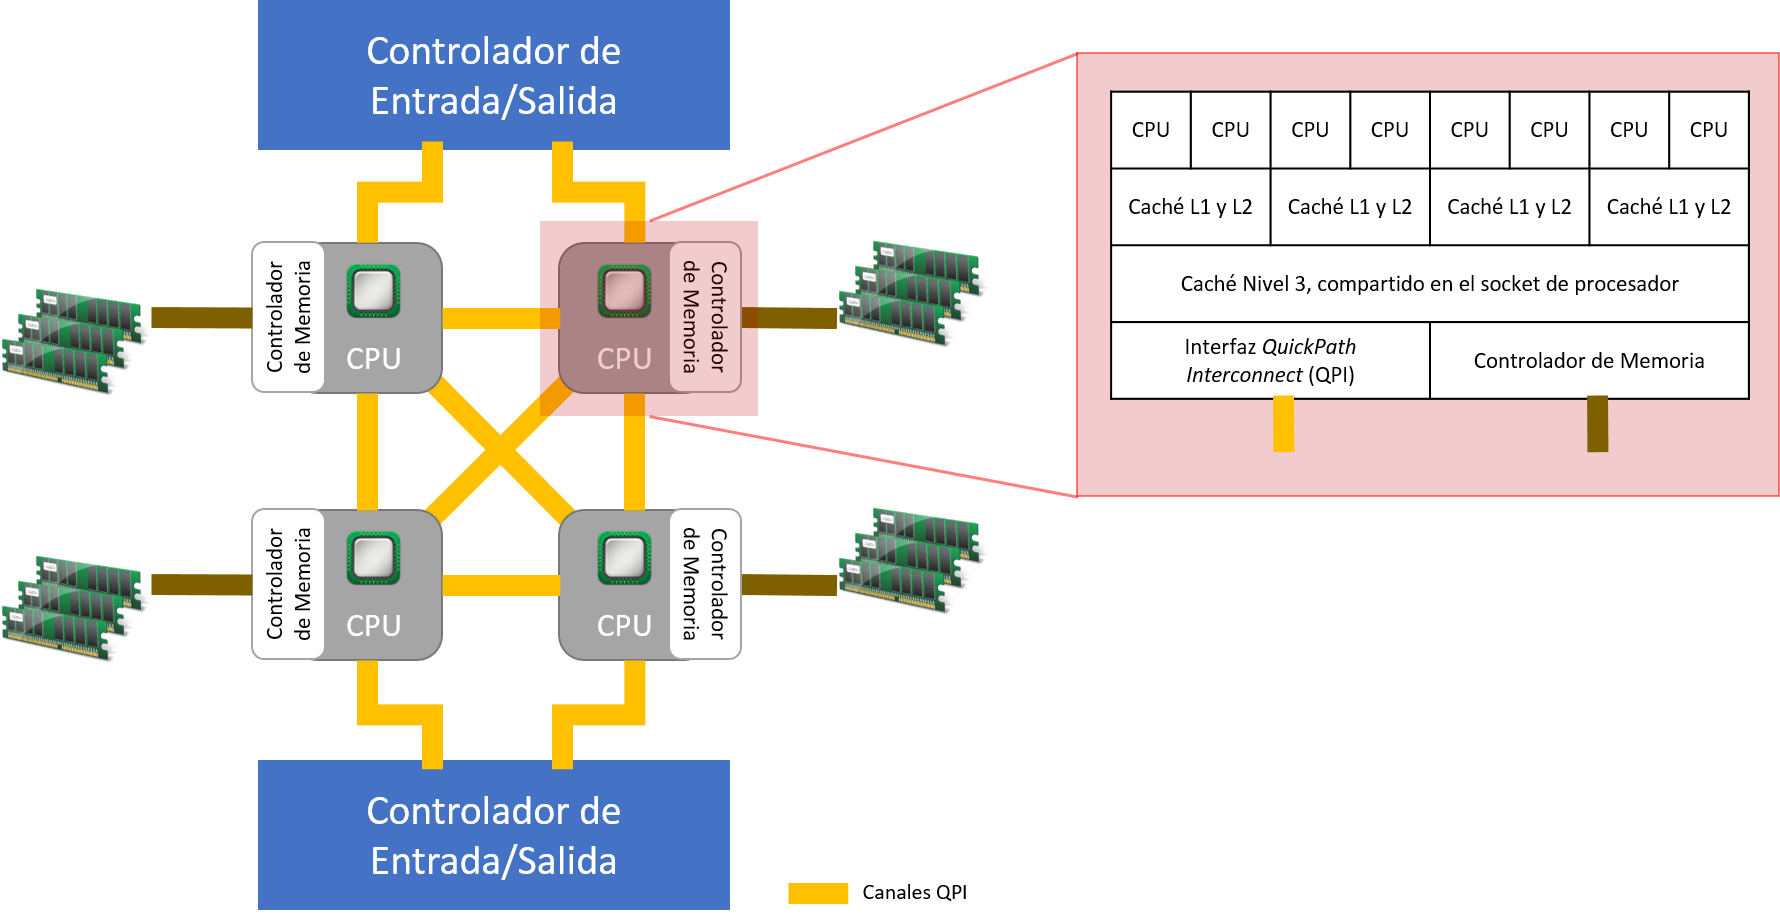
\includegraphics[scale=.5]{imagenes/quickpath2.png}
	\caption{Diseño organizacional de los componentes de sistema en una arquitectura estándar \emph{QuickPath} de Intel.}
	\label{fig:quickpath}
\end{figure}

El esquema \emph{QuickPath} postula una reformación arquitectural de los componentes principales de un sistema \ref{fig:quickpath}. En ésta propuesta, las distintas unidades de procesamiento (CPU) están interconectadas por canales de comunicación especiales denominados \emph{Intel QuickPath Interconnect - QPI} que son conexiones punto a punto entre CPU de enorme velocidad de transferencia (llegando hasta 25 GB/s en canales con variantes unidireccional o bidireccional). En línea para aprovechar esta nueva arquitectura, Intel® propone una serie de modificaciones al tradicional protocolo MESI, construyendo el denóminado protocolo \textbf{MESIF} que es una evolución del primero, flexibilizando los protocolos de coherencia de caché al incorporar un nuevo estado para las lineas de caché (\textbf{F} - \emph{Forward}) dotando así de mayor eficiencia y velocidad de acción entre procesadores al ser una comunicación directa.

Por otro lado, en la arquitectura \emph{QuickPath} cada CPU dispone de su propio controlador de memoria y de un banco de memoria de acceso próximo. Dicho diseño se denomina un nodo \textbf{NUMA} de sus siglas en inglés \emph{\textbf{N}on \textbf{U}niform \textbf{M}emory \textbf{A}ccess} [CITA A NUMA] la que permite a las CPU de cada nodo NUMA disponer de un banco de memoria con un acceso garantizado más rápido que al que se tendría acceso en una arquitectura tradicional. El enfoque \emph{NUMA} se aprovecha del principio de localidad de memoria \cite{paper:memorylocality}, por la cual postula que los datos son separables en su acceso por las distintas CPU, logrando así mayor velocidad en el acceso a la memoria, y menor problemas de coherencia de la misma por modificaciones entre CPUs.

El trabajo de Intel® va más allá. Conscientes de la necesidad de herramientas y utilidades para analizar la verdadera performance que provee ésta arquitectura, Intel® provee unidades de monitoreo de performance embebidas en sus procesadores (o \textbf{PMU}, por sus siglas en ingles \emph{\textbf{P}erformance} \textbf{M}onitoring \textbf{U}nit) que son componentes de hardware incorporado a los sistemas que permiten la inspección de operaciones a nivel de comunicación entre componentes del sistema directamente. A éste tipo de análisis se denomina \emph{estudios de Perfomance Counters} dado que para poder realizar una medición, el fabricante de la PMU provee una colección de posibles eventos a colectar, con significaciones puntuales cada uno.

\begin{defn}[ver \cite{KAR00}] \textbf{Performance Counters} son identificadores de máquina que permiten cuantificar determinados eventos a nivel de hardware, como lecturas de caché, corrección de líneas de caché, comunicación de protocolos de coherencia, etc. Usados para analizar el comportamiento de ciertas unidades de hardware y que conforman la base de las herramientas de profiling moderno para el rastreo en el comportamiento de funciones de un sistema.
\end{defn}

La Intel® \emph{QuickPath Architecture} implementa un modelo de 5 capas (Ver fig. \ref{fig:5layersqpi}) para la comunicación de datos entre los núcleos de procesamiento (Similar al espíritu del modelo OSI). De dicho modelo, para la detección de comunicación de aplicaciones son muy significativos los niveles de: \textbf{Protocolo}, al asociar tareas del paso de paquetes, aplicación del protocolo MESIF y de los mecanismos de SNOOP para control y coherencia de líneas de caché, y \textbf{Link}, para el reconocimiento de mecanismos de corrección de errores y recuperación a lo largo de la transmisión de datos entre dispositivos, y para el llamado esquema de \emph{Crédito/Débito} desarrollado por el mismo fabricante que permite trasmisiones de datos confiables entre componentes.

\begin{figure}[!h]
	\centering
	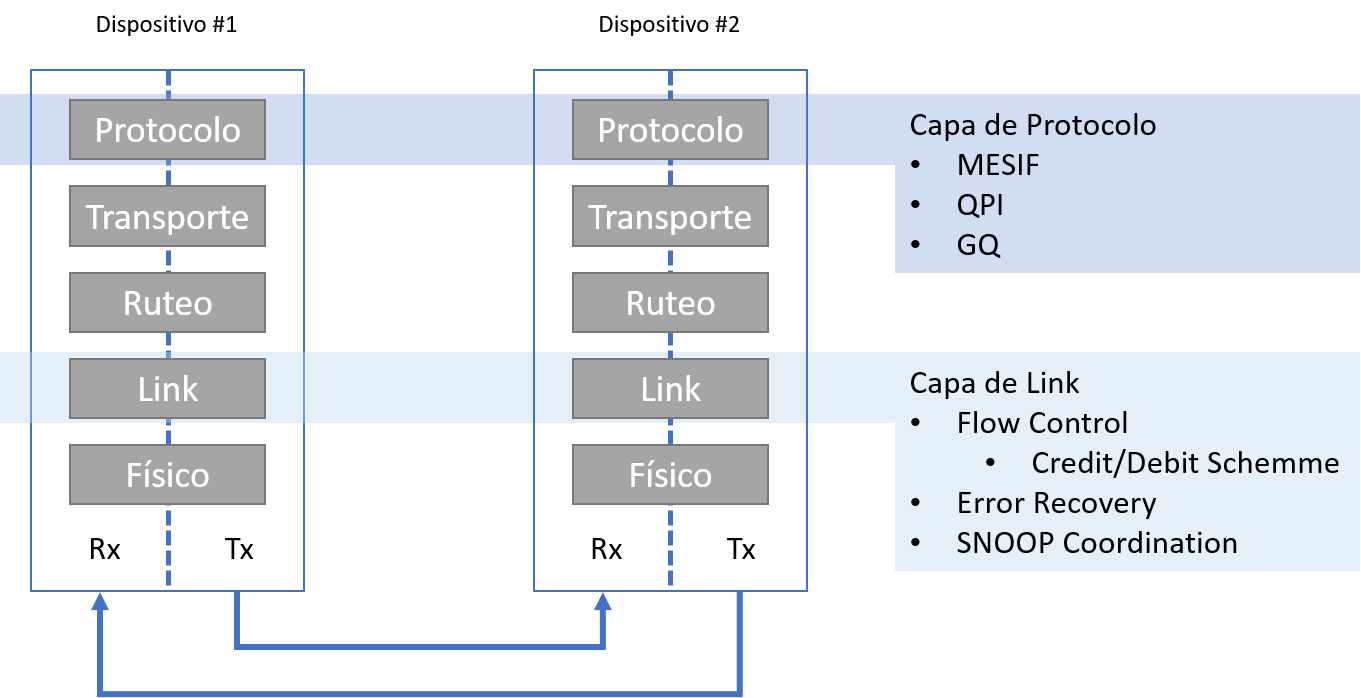
\includegraphics[scale=.5]{imagenes/5layersqpi.png}
	\caption{Diagrama de las 5 capas implementadas en la Intel® \emph{QuickPath Architecture} ilustrando los niveles de control de distintas componentes y protocolos importantes del sistema.}
	\label{fig:5layersqpi}
\end{figure}

El estudio de \emph{performance counters} corresponde a uno de los análisis de más bajo nivel realizables en pos de obtener datos que representen la forma fiel la comunicación entre componentes del sistema. Ello lo hace también un estudio dificultoso de realizar pues amerita un gran conocimiento de la arquitectura puntual sobre el sistema que se desea estudiar, pero de enorme valor para valerse de información sobre la verdadera cuota de comunicación inherente a un caso de estudio.

\section{Especificación y Captura de Eventos}
Para definir el marco conceptual de la prueba, se debe mantener presente el contexto de la hipótesis que fundamenta la misma. En éste caso, la motivación de éste estudio está en línea con entender el comportamiento de un consumo concurrente en una estructura socket, o más precisamente, ver cómo una instancia de una primitiva de sincronización --un spinlock-- se comporta a nivel de actividad de hardware en un escenario multithread. En ese escenario, se busca estudiar cómo se manifestaría la expresión de los protocolos de coherencia de cache bajo circunstancias de ejecución en un escenario mutiprocesador que podrían dar cuenta de que el mal desempeño general del caso de estudio tiene sus origines en los mismos sistemas de coordinación de bajo nivel del sistema.

\subsection{Arquitectura de la máquina para las pruebas}
Siguiendo el caso de prueba evaluado a lo largo de la investigación, se inspeccionará el caso de estudio de saturación de un socket UDP en el equipo servidor multicore para pruebas (Ver fig. \ref{fig:hwspecs}). En éste caso, se cuenta con un equipo placa Dell Inc. 00NH4P A07, provisto de dos CPU Intel Xeon 5600 2.8Ghz, dotado de 6 cores cada uno. Cada CPU dispone de hasta tres niveles de cache de 192 kb, 1536kb y 12288kb respectivamente, que combinados con tres memorias de 4096MB (DDR3 1333MHz) cada uno, conforman 2 nodos NUMA, con un monto total de 24GB de memoria. Una configuración que es precisamente de la familia \emph{Intel QuickPath Architecture} y es enfocada a servidores multicpu \cite{report:intelxeon5600, manual:intelxeon5600}.

\begin{figure}[!h]
	\centering
	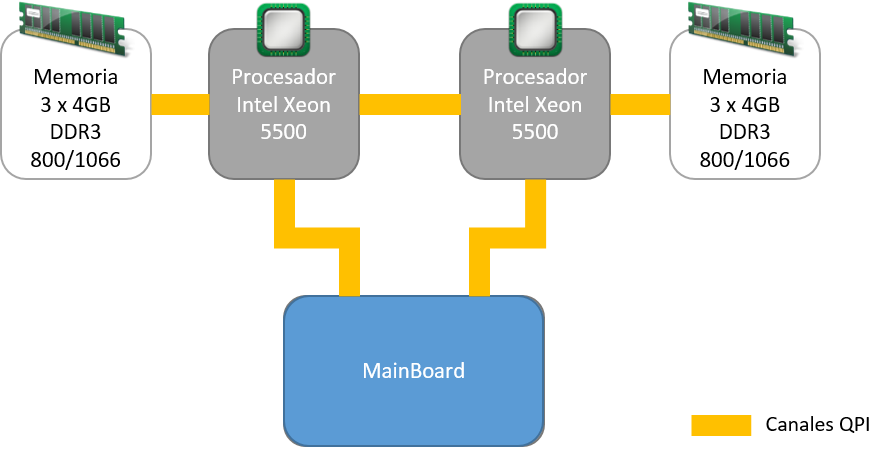
\includegraphics[scale=.75]{imagenes/arch24Cores.png}
	\caption{Esquema de arquitectura interna del esquipo servidor multicore sobre el que se realizan las pruebas de \emph{performance counters}.}
	\label{fig:hwspecs}
\end{figure}

Para inspeccionar el sistema donde se evalúan las pruebas en detalle en busca de componentes de monitoreo disponibles se utilizó la utilidad \emph{libpfm4}\footnote{\url{http://www.bnikolic.co.uk/blog/hpc-prof-events.html}} que corresponde a una herramienta confeccionada para recuperar información sobre los códigos de inspección de eventos de performance counters de un sistema y de las PMU disponibles en el mismo. De ello, se da cuenta de que para el modelo de procesador presente se dispone de 5 unidades de PMU disponibles, separables en 3 grupos (Ver código \ref{code:pmuavailable}):
\begin{description}
\item[PMU Genéricas] Incluyen a \verb=perf= y  \verb=perf_raw=. Disponen de las especificaciones estándar de \emph{performance counters} de la línea del software \emph{Perf}, lo cual las hace poco exactas en los valores descritos por cada evento y no necesariamente fieles a su especificación pues dependen en gran parte de que el fabricante sea riguroso en su implementación.
\item[PMU x86] PMU generacional de Intel para la línea x86 de Intel que incluye a \verb=ix86arch=. Dispone de eventos comunes a dicha línea de procesadores por lo que no da soporte específico para la arquitectura \emph{QuickPath} ni del funcionamiento multiprocesador.
\item[PMU westmere] PMU específicas de la línea Westmere [AKA UNA CITA] que soporta la base del desarrollo de la \emph{Intel QuickPath Architecture}, incluyendo a \verb=wsm_dp= y \verb=wsm_unc=. Es el nivel más exacto de PMU que provee el fabricante con los eventos más especificos y documentados del sistema, por lo que es la PMU más importante a la hora de colectar eventos.
\end{description}

\vspace{1pc}
\begin{lstlisting}[style=BashInputStyle, label={code:pmuavailable}, caption={Listado de \emph{PMUs} disponibles en el sistema, recuperado con la herramienta \emph{libpfm4}.}, captionpos=b]
	Detected PMU models:
[18, ix86arch, "Intel X86 architectural PMU", 6 events, 1 max encoding, 7 counters, core PMU]
[51, perf, "perf_events generic PMU", 104 events, 1 max encoding, 0 counters, OS generic PMU]
[53, wsm_dp, "Intel Westmere DP", 91 events, 2 max encoding, 7 counters, core PMU]
[54, wsm_unc, "Intel Westmere uncore", 52 events, 1 max encoding, 9 counters, uncore PMU]
[114, perf_raw, "perf_events raw PMU", 1 events, 1 max encoding, 0 counters, OS generic PMU]
\end{lstlisting}

\subsection{Metodología de captura de eventos}
Para la especificación de la captura de eventos resulta imprescindible prestar especial atención a la arquitectura interna que soporta la comunicación interprocesador del sistema. En la figura \ref{fig:hwcomm} se da cuenta de los canales de comunicación que dispone el sistema estudiado, haciendo un acercamiento a cada unidad lógica de procesamiento, núcleo de cada nodo NUMA.

\begin{figure}[!h]
	\centering
	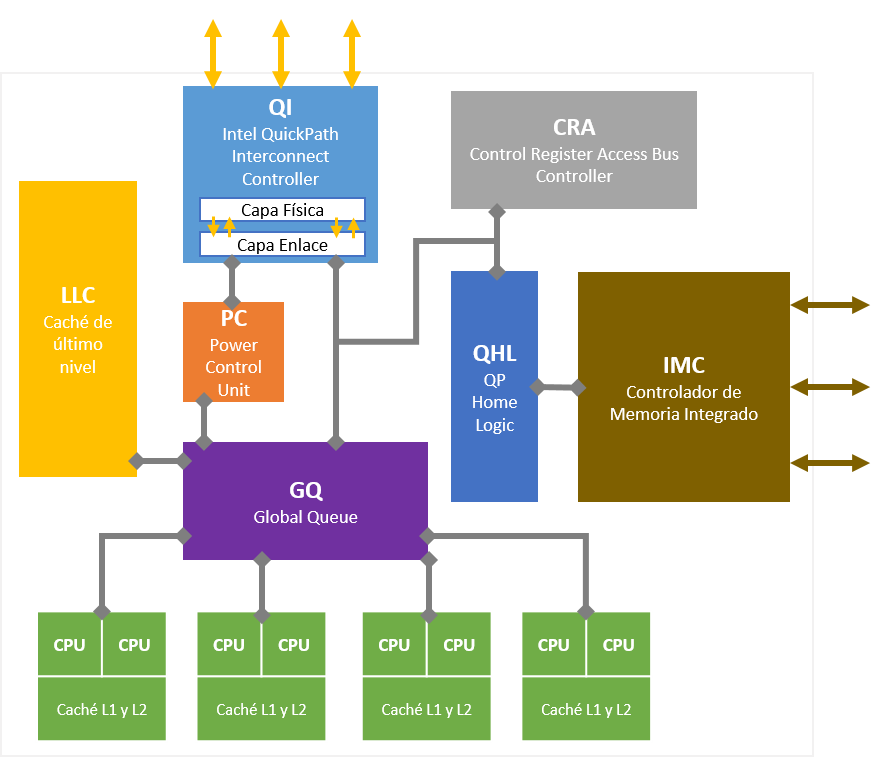
\includegraphics[scale=.8]{imagenes/QuickPathChannels.png}
	\caption{Esquema de arquitectura interna del equipo servidor multicore estudiado, ilustrando las vías de comunicación del procesador que da cuenta de los principales puntos de alta comunicación en el escenario de \textit{cache bouncing} por contención de valores.}
	\label{fig:hwcomm}
\end{figure}

La figura \ref{fig:hwcomm} da cuenta de los distintos puntos en que se pueden suceder escenarios de congestión dados ya sea por un alto nivel de uso de los protocolos de coordinación de memoria o por un alto tráfico de comunicación entre CPUs. Dichos canales de comunicación podemos resumirlos en las siguientes funciones dedicadas de la arquitectura estudiada, que a su vez están asociadas a ciertos \emph{performance counters} del sistema:

\begin{itemize}
\item Uso de los canales \emph{Intel QuickPath QPI}
\item Acciones del protocolo \emph{SNOOP}
\item Pasos de datos entre distintos caché y memoria
\item Transiciones del protocolo \emph{MESI(F)}
\end{itemize}

Con ello en mente, se consultó el manual oficial del fabricante \cite{manual:bigbigevents} en búsqueda de documentación acerca de eventos disponible en el sistema que se relacionaran a las operaciones antes descritas. De dicha documentación, combinado con la utilidad \emph{libpfm4} para la recolección de eventos disponibles se colectaron un total de 143 eventos cada uno con hasta 6 variantes de configuración, dando en total casi 500 posibles eventos a estudiar. En este escenario es preciso acotar los eventos a considerar, de acuerdo a los 4 criterios antes descritos.


%[[[Hablar un poco de dicha busqueda y del manual]]]]

Finalmente, siguiendo los 4 criterios de puntos problemáticos a estudiar se construyó una selección de eventos a considerar resumida en la tabla \ref{table:eventos}. Los eventos están divididos en dos grupos: \textbf{QPI/GQ/Cache} para eventos relacionados con movimiento o traslación de datos entre distintas unidades de hardware, y \textbf{LinkLayer} para eventos referidos a protocolos de consistencia y sincronización que son pertinentes a la capa de corrección en el esquema de capas del \emph{Quickpath}.

\begin{table}[h!]
\centering
\begin{tabular}{l|l}
\multicolumn{1}{c|}{{\bf QPI/GQ/CACHE}} & \multicolumn{1}{c}{{\bf LinkLayer}} \\ \hline
{ UNC\_GQ\_DATA\_FROM} & SNOOPQ\_REQUESTS \\
{ UNC\_GQ\_DATA\_TO} & SNOOPQ\_REQUESTS\_OUTSTANDING \\
{ UNC\_QHL\_REQUESTS} & SNOOP\_RESPONSE \\
{ L1D} & UNC\_QPI\_RX\_NO\_PPT\_CREDIT \\
{ L2\_DATA\_RQSTS} & UNC\_QPI\_TX\_STALLED\_MULTI\_FLIT \\
{ UNC\_LLC\_HITS} & UNC\_QPI\_TX\_STALLED\_SINGLE\_FLIT \\
{ UNC\_LLC\_MISS} & UNC\_SNP\_RESP\_TO\_LOCAL\_HOME \\
{ UNC\_LLC\_LINES\_IN} & UNC\_SNP\_RESP\_TO\_REMOTE\_HOME \\
{ UNC\_LLC\_LINES\_OUT} & UNC\_IMC\_RETRY
\end{tabular}
\caption{Total de eventos inspeccionados y estudiados en el caso de estudio de consumo concurrente sobre sockets UDP.}
\label{table:eventos}
\end{table}

Con los eventos a colectar más claros, el siguiente paso consiste en conseguir los códigos de registro para la adquisición de cada evento. Un código de registro sigue una nomenclatura dada por el fabricante de la PMU y no guarda relación semántica con el valor que reporta, pero es la única referencia para indicar al software de recolección de datos el evento de interés a estudiar. Para ello, se confeccionó una herramienta\footnote{\url{https://github.com/sebablasko/libpfm4PerformanceEventParser}} para la obtención de los códigos de registros de cada evento de interés la cual trabajando en conjunto con \emph{libpfm4} es capaz de parsear datos del sistema para generar una colección de códigos de registro asociados a eventos de hardware en formato \verb=JSON=, según los cuales se tiene una correcta representación del nivel de saturación y uso de los componentes. Con el \verb=JSON= generado, se pueden hacer mediciones de forma sencilla usando la herramienta \verb=stat= de \emph{Perf} para generar un reporte de la cantidad de veces que se registre actividad en el evento estudiado, especificado en la misma herramienta.

\vspace{1pc}
\begin{lstlisting}[style=BashInputStyle, breaklines=true, captionpos=b, caption={Ejemplo de uso de Perf para colectar datos de una colección de eventos. En éste caso se configura para colectar datos de 2 eventos y dejar el reporte en un archivo de salida.}]
	# perf stat -e r53003c,r5300c0 -o resultado.txt -- ./programa
\end{lstlisting}

Finalmente, de los output de Perf se pueden estudiar los resultados finales de la comunicación efectiva generada a lo largo de la prueba.

\section{Metodología de Experimentación}
Para poder comprender mejor las tendencias de comportamiento de los distintos eventos en cada instancia de prueba con una determinada configuración de threads, se confeccionó un experimento donde se evaluaron 3 escenarios de consumo para comparar sus resultados\footnote{\url{https://github.com/sebablasko/Test_PerformanceCounters}}:

\begin{enumerate}
\item Lectura concurrente desde un dispositivo virtual como \verb=dev_null=. Para ilustrar el comportamiento en el caso de menor sobrecarga en lectura concurrente al ser un dispositivo libre de barreras de bloqueo.
\item Lectura exclusiva desde un socket UDP. En éste caso se consume la cuota definida en el caso de estudio por sockets con acceso exclusivo, distribuyendo la carga entre ellos con sólo 1 thread por socket. 
\item Lectura concurrente desde un socket UDP. Precisamente el caso de estudio evaluado a lo largo de toda la investigación.
\end{enumerate}

Así se puede tener un punto de comparación del fenómeno que se manifiesta en escenarios de lectura concurrente sobre un socket, y que no se manifiesta en otros escenarios.

Para la recolección de datos se empleó nuevamente el software \emph{Perf} para la administración y control de la PMU del sistema. Al igual que en el caso de estudio original se evalúan configuraciones de 1, 2, 4, 8, 16, 24, 36, 48, 64 y 128 threads contemplando un total de 60 repeticiones del proceso de captura para cada configuración de prueba. En la recolección de datos se define $T_i$ a la tupla que agrupa los resultados de cada una de las 60 repeticiones para una configuración de la prueba empleando $i$ hilos.

\begin{equation}
\label{eq:tupla1}
T_i = \left\{ T_{i,1},T_{i,2},T_{i,3}, \dots ,T_{i,59}, T_{i,60}\right\} 
\end{equation}

Con las muestras totales para cada configuración, se pueden determinar representantes estadísticos que nos permitan ilustrar el valor de cada configuración. Para éste propósito se emplea el calculo del promedio simple entre las muestras.

\begin{equation}
\label{eq:promedio}
\overline{T_{i}} = \frac{T_{i,1}+T_{i,2}+T_{i,3}+ \dots +T_{i,59}+ T_{i,60}}{60}
\end{equation}

Finalmente, se construye con para cada evento estudiado un set de registros que guardan el valor promedio de cada evaluación en una determinada configuración de hilos de ejecución.

\begin{equation}
\label{eq:tupla2}
Evento_j = \left(\overline{T_{1}}, \overline{T_{2}}, \overline{T_{4}}, \overline{T_{6}}, \overline{T_{8}}, \overline{T_{16}}, \overline{T_{24}}, \overline{T_{36}}, \overline{T_{48}}, \overline{T_{60}}\right)
\end{equation}

De ésta manera, se pueden hacer análisis más simples sobre las variables aleatorias $Evento_j$ que permita una simple comparación entre cada una de los 3 escenarios de evaluación estipulados.

\section{Resultados}
Dada la enorme cantidad de resultados obtenidos en el proceso de inspección de los \emph{performance counters}, se presentan sólo aquellos resultados con comportamiento interesante registrado en el caso de prueba.

Los resultados se han agrupado en 8 categorías para facilitar la asociación de comportamientos y de elementos analizados: Comportamiento de caché de datos de nivel 1, caché de nivel 2, último nivel de caché y banco de memoria, fallo en predicción de procesamiento, solicitudes fuera del core, comunicación por canales de la arquitectura \emph{Quickpath} y finalmente actividad de coordinación por protocolos \emph{SNOOP} y \emph{MESIF}.

\begin{figure}[ph!]
\centering
\subfigure[]{
	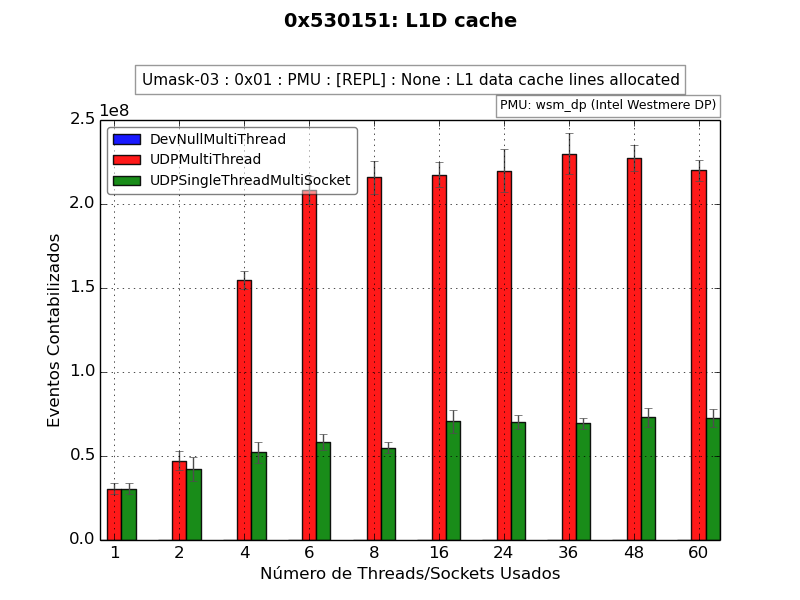
\includegraphics[width=.47\textwidth]{resultados/pcounters/r530151.png}
	\label{fig:pcounterL1a}
}
\subfigure[]{
	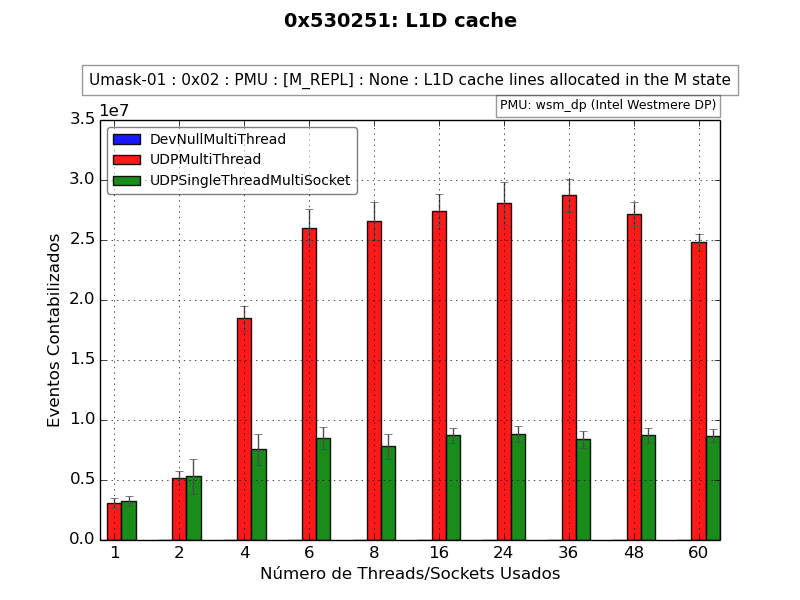
\includegraphics[width=.47\textwidth]{resultados/pcounters/r530251.png}
	\label{fig:pcounterL1b}
}
\subfigure[]{
	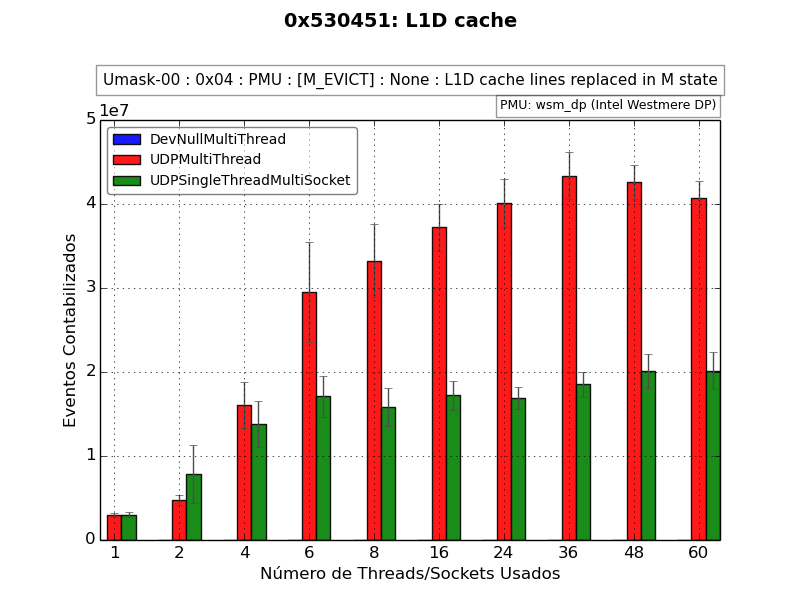
\includegraphics[width=.47\textwidth]{resultados/pcounters/r530451.png}
	\label{fig:pcounterL1c}
}
\subfigure[]{
	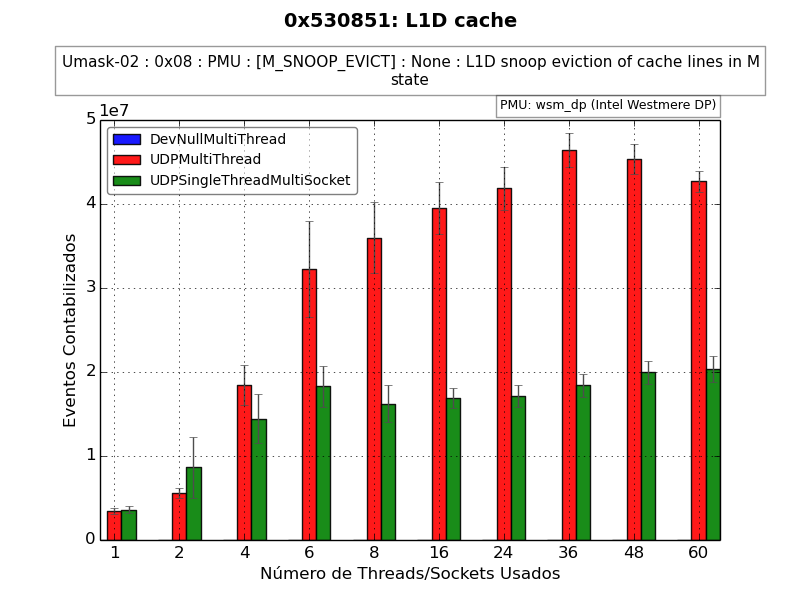
\includegraphics[width=.47\textwidth]{resultados/pcounters/r530851.png}
	\label{fig:pcounterL1d}
}
\caption{Resultados asociados al comportamiento del caché de datos de primer nivel.}
\label{fig:pcounterL1}
\end{figure}

\begin{figure}[ph!]
\centering
\subfigure[]{
	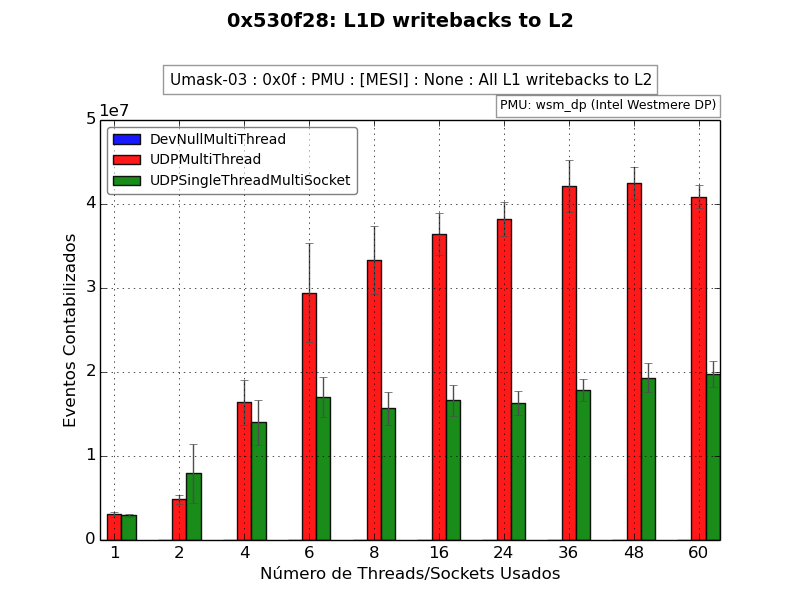
\includegraphics[width=.47\textwidth]{resultados/pcounters/r530f28.png}
	\label{fig:pcounterMESIFa}
}
\subfigure[]{
	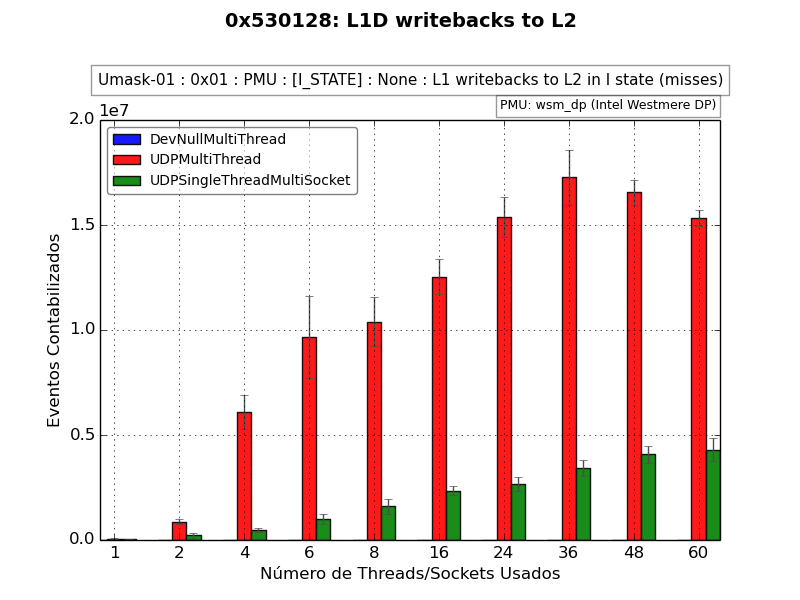
\includegraphics[width=.47\textwidth]{resultados/pcounters/r530128.png}
	\label{fig:pcounterMESIFb}
}
\caption{Resultados asociados al comportamiento del protocolo MESIF.}
\label{fig:pcounterMESIF}
\end{figure}

\begin{figure}[ph!]
\centering
\subfigure[]{
	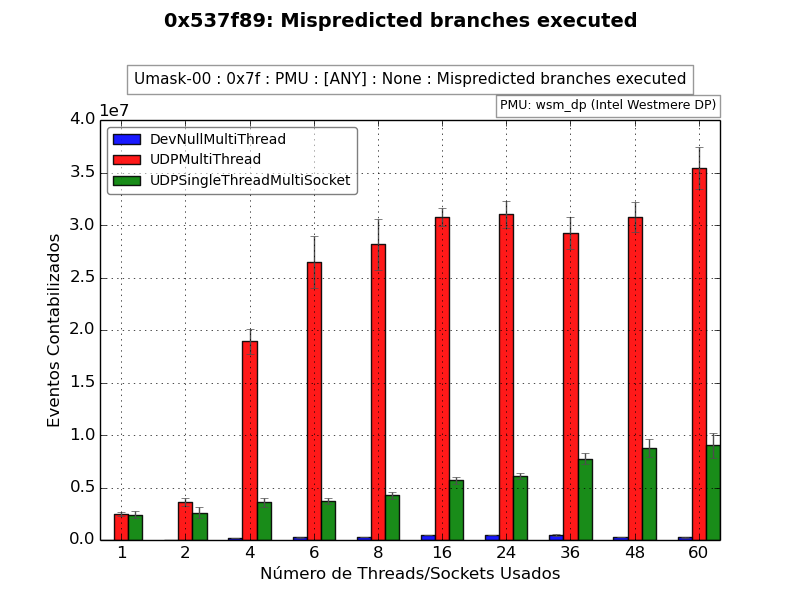
\includegraphics[width=.47\textwidth]{resultados/pcounters/r537f89.png}
	\label{fig:pcounterMissBranchPredictiona}
}
\subfigure[]{
	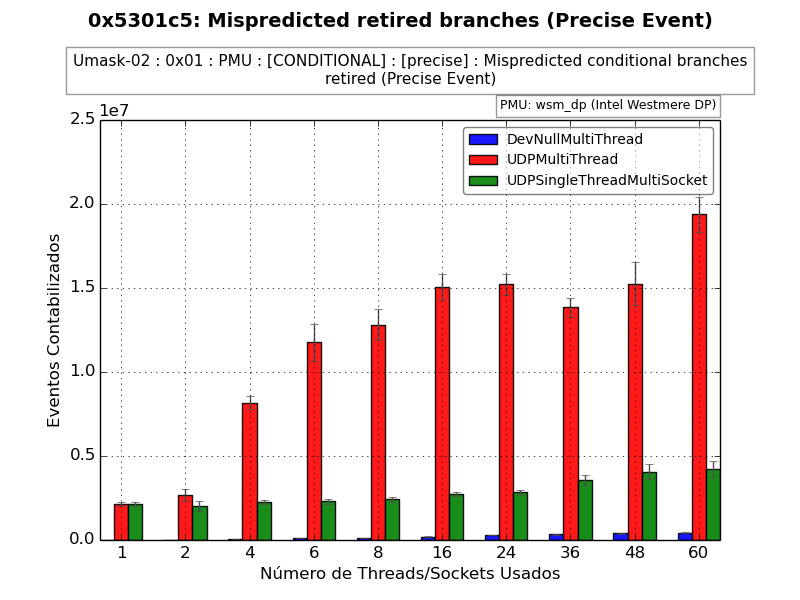
\includegraphics[width=.47\textwidth]{resultados/pcounters/r5301c5.png}
	\label{fig:pcounterMissBranchPredictionb}
}
\caption{Resultados asociados al fenómeno de fallo en predicción de ejecución del procesador.}
\label{fig:pcounterMissBranchPrediction}
\end{figure}


\begin{figure}[ph!]
\centering
\subfigure[]{
	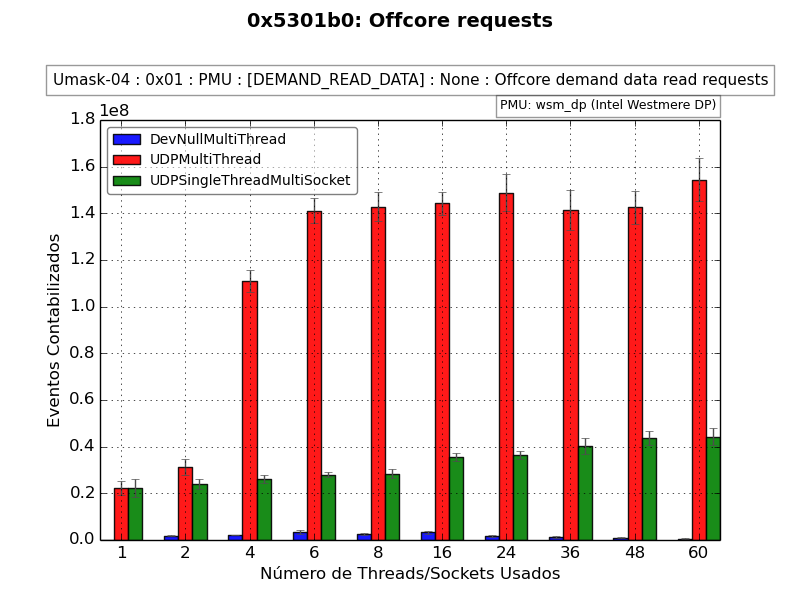
\includegraphics[width=.47\textwidth]{resultados/pcounters/r5301b0.png}
	\label{fig:pcounterOFFCorea}
}
\subfigure[]{
	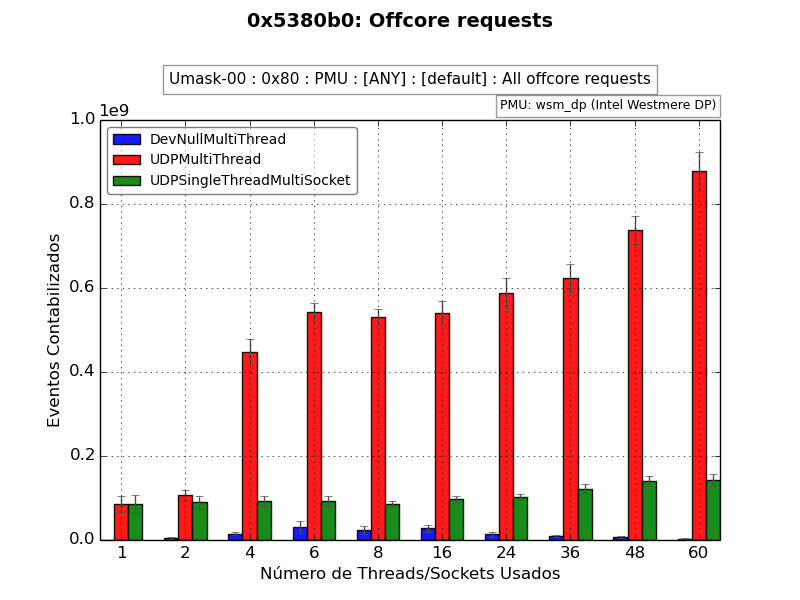
\includegraphics[width=.47\textwidth]{resultados/pcounters/r5380b0.png}
	\label{fig:pcounterOFFCoreb}
}
\subfigure[]{
	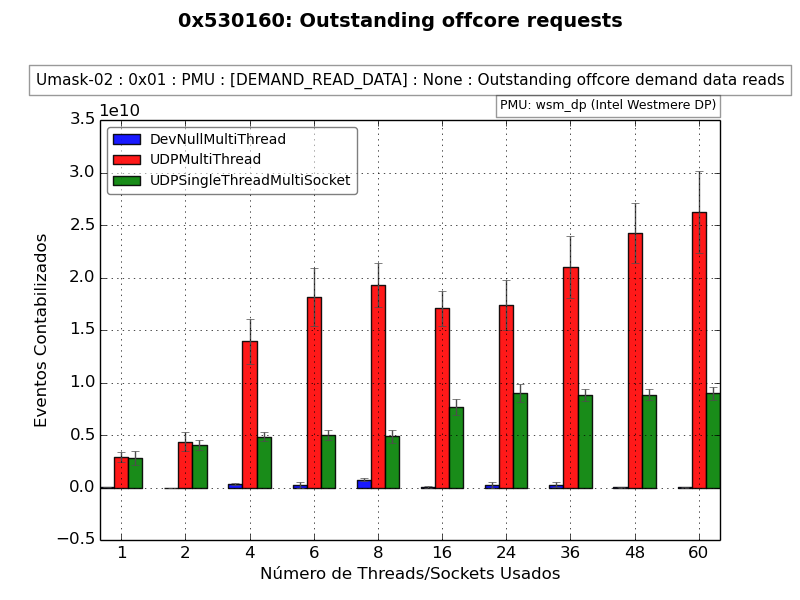
\includegraphics[width=.47\textwidth]{resultados/pcounters/r530160.png}
	\label{fig:pcounterOFFCorec}
}
\caption{Resultados asociados al comportamiento de fallo en solicitud de datos de un core.}
\label{fig:pcounterOFFCore}
\end{figure}

\begin{figure}[ph!]
\centering
\subfigure[]{
	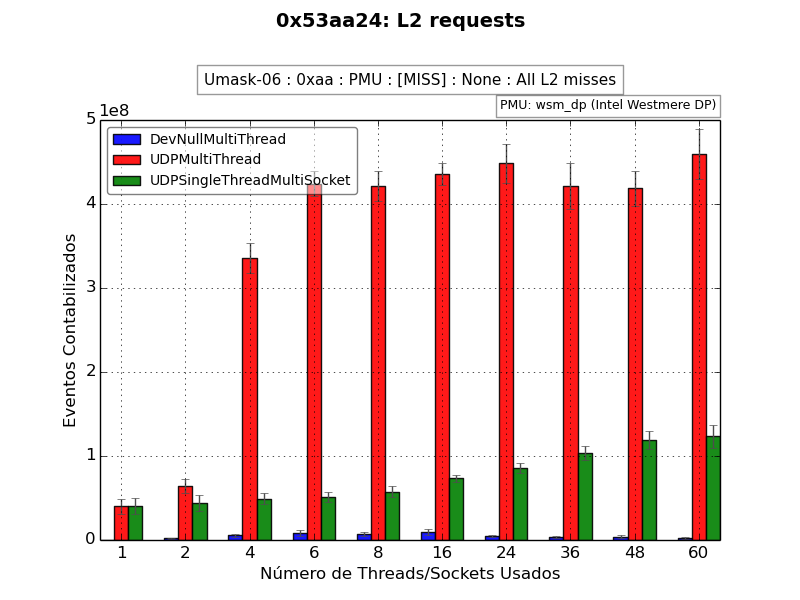
\includegraphics[width=.47\textwidth]{resultados/pcounters/r53aa24.png}
	\label{fig:pcounterL2a}
}
\subfigure[]{
	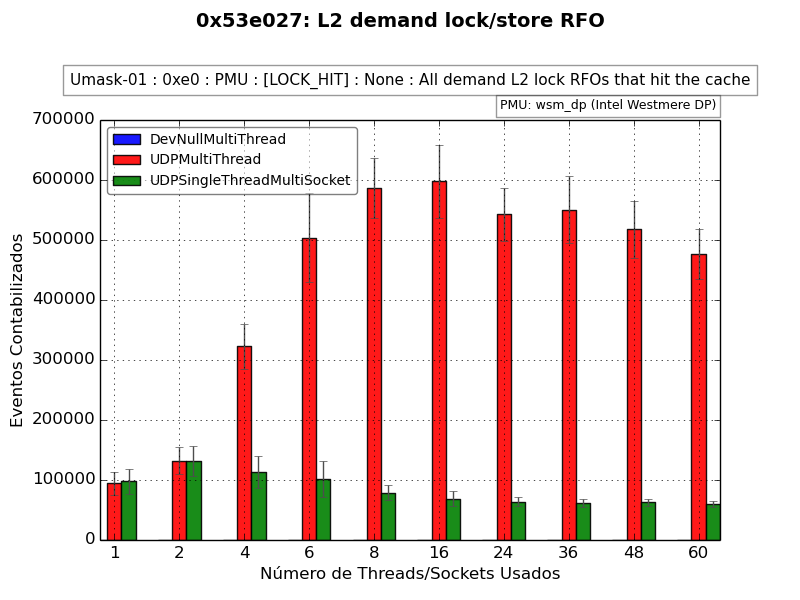
\includegraphics[width=.47\textwidth]{resultados/pcounters/r53e027.png}
	\label{fig:pcounterL2b}
}
\subfigure[]{
	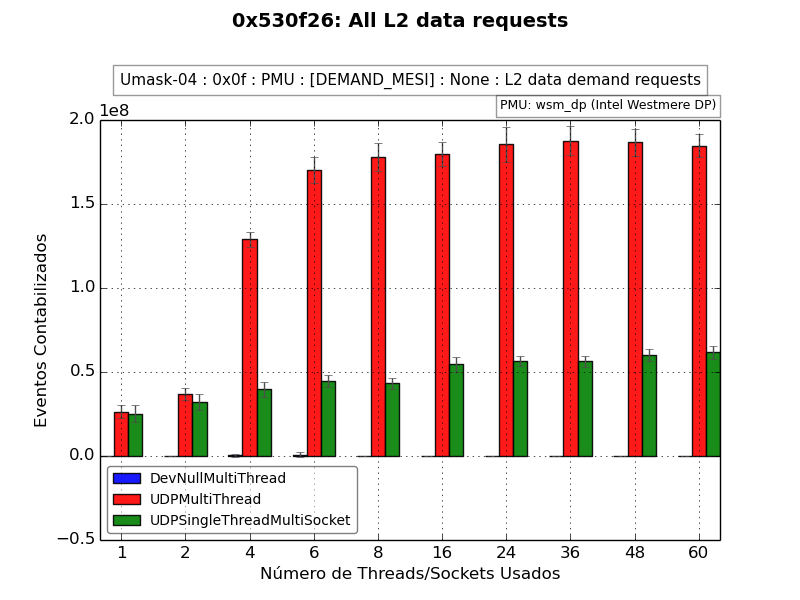
\includegraphics[width=.47\textwidth]{resultados/pcounters/r530f26.png}
	\label{fig:pcounterL2c}
}
\subfigure[]{
	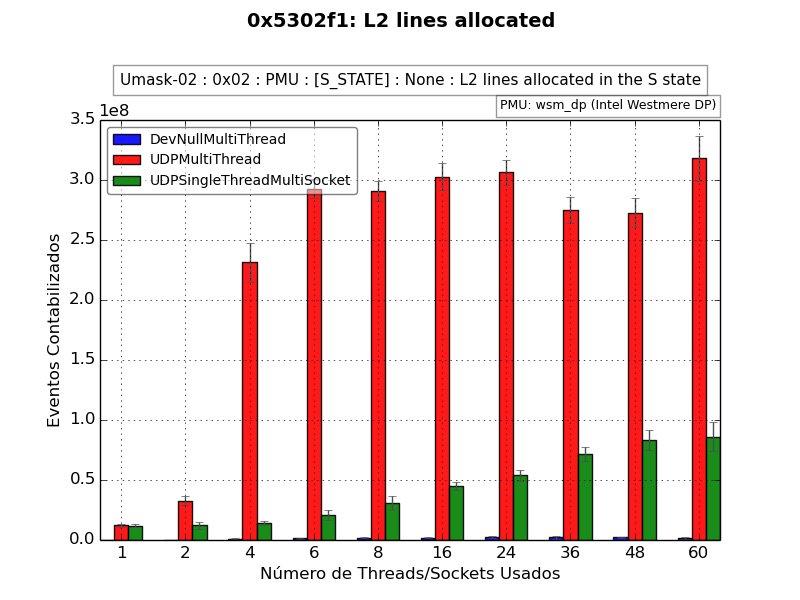
\includegraphics[width=.47\textwidth]{resultados/pcounters/r5302f1.png}
	\label{fig:pcounterL2d}
}
\subfigure[]{
	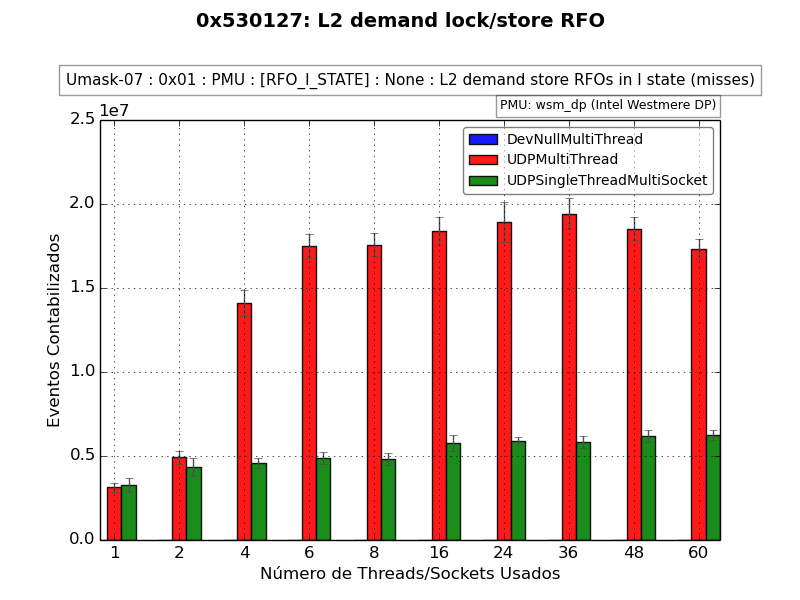
\includegraphics[width=.47\textwidth]{resultados/pcounters/r530127.png}
	\label{fig:pcounterL2e}
}
\caption{Resultados asociados al comportamiento del caché de segundo nivel.}
\label{fig:pcounterL2}
\end{figure}


\begin{figure}[ph!]
\centering
\subfigure[]{
	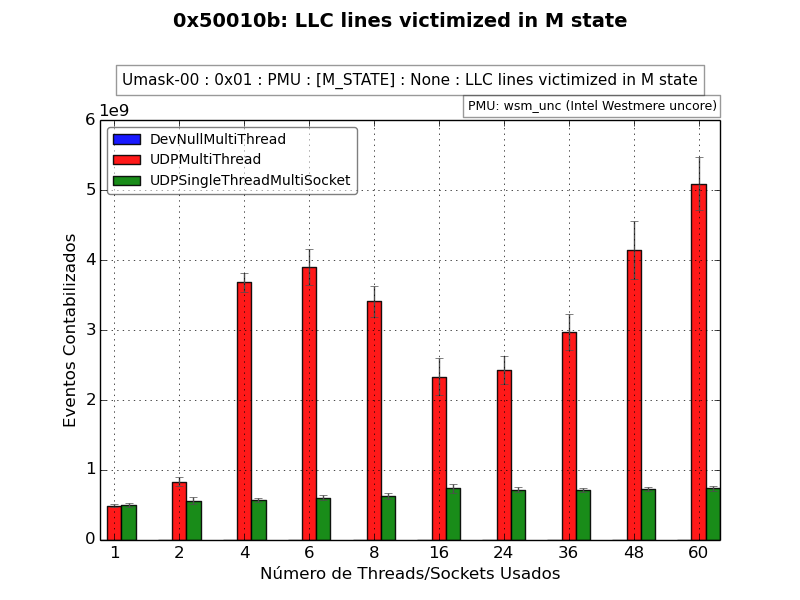
\includegraphics[width=.47\textwidth]{resultados/pcounters/r50010b.png}
	\label{fig:pcounterLLCa}
}
\subfigure[]{
	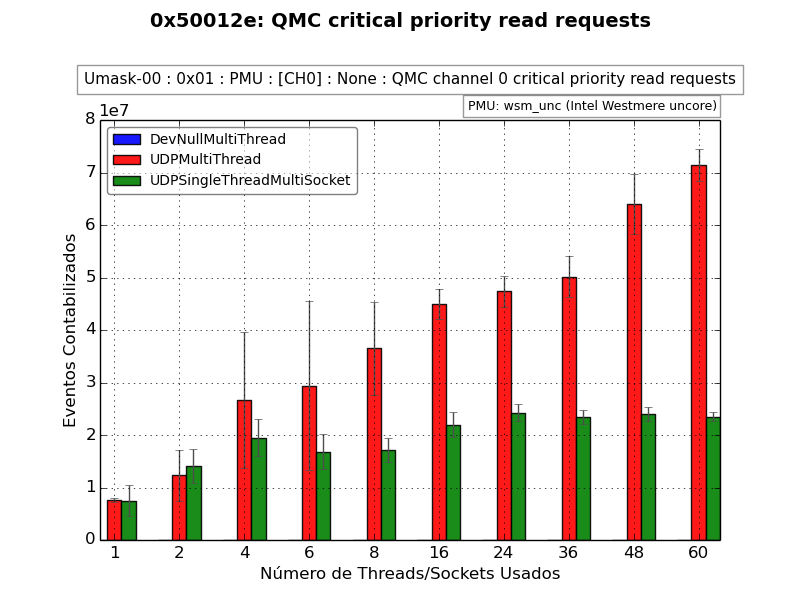
\includegraphics[width=.47\textwidth]{resultados/pcounters/r50012e.png}
	\label{fig:pcounterLLCb}
}
\subfigure[]{
	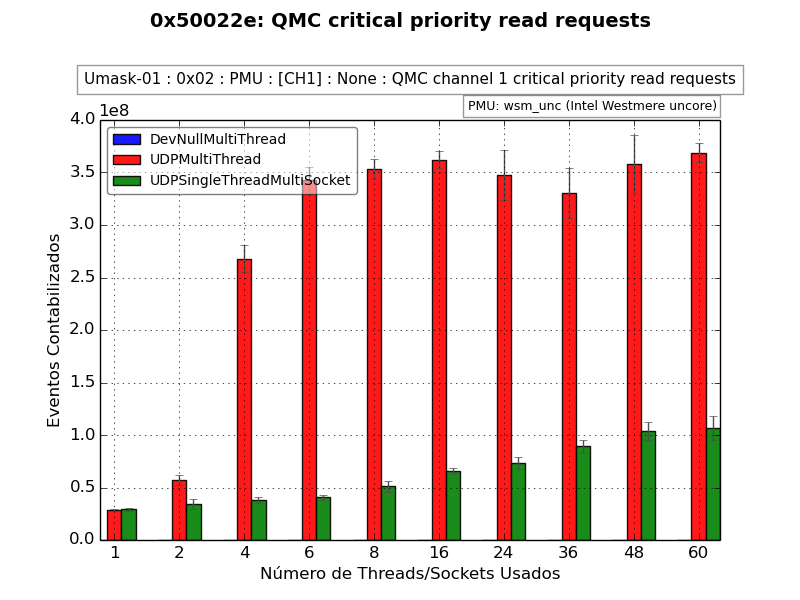
\includegraphics[width=.47\textwidth]{resultados/pcounters/r50022e.png}
	\label{fig:pcounterLLCc}
}
\subfigure[]{
	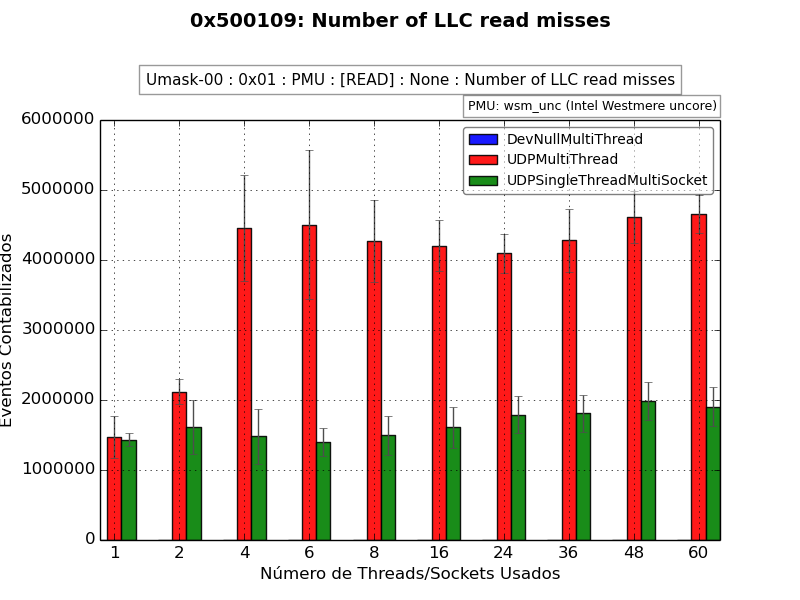
\includegraphics[width=.47\textwidth]{resultados/pcounters/r500109.png}
	\label{fig:pcounterLLCd}
}
\subfigure[]{
	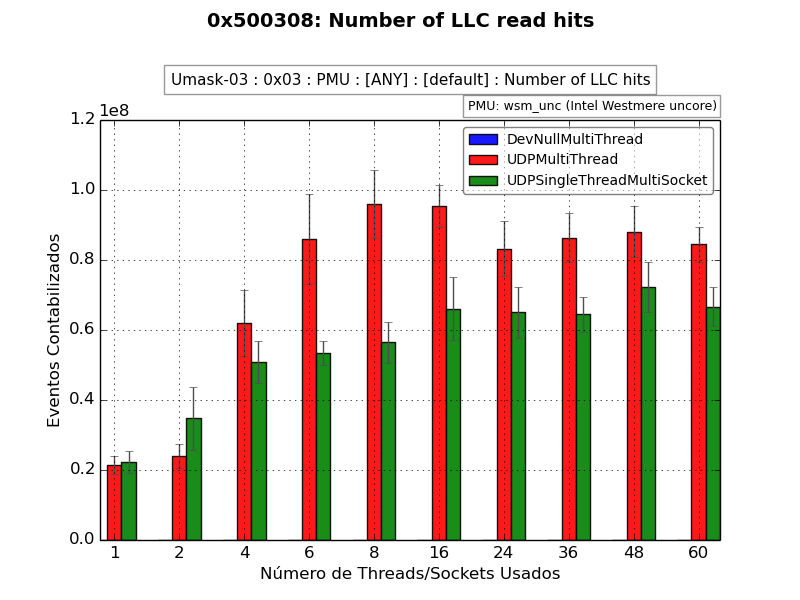
\includegraphics[width=.47\textwidth]{resultados/pcounters/r500308.png}
	\label{fig:pcounterLLCe}
}
\subfigure[]{
	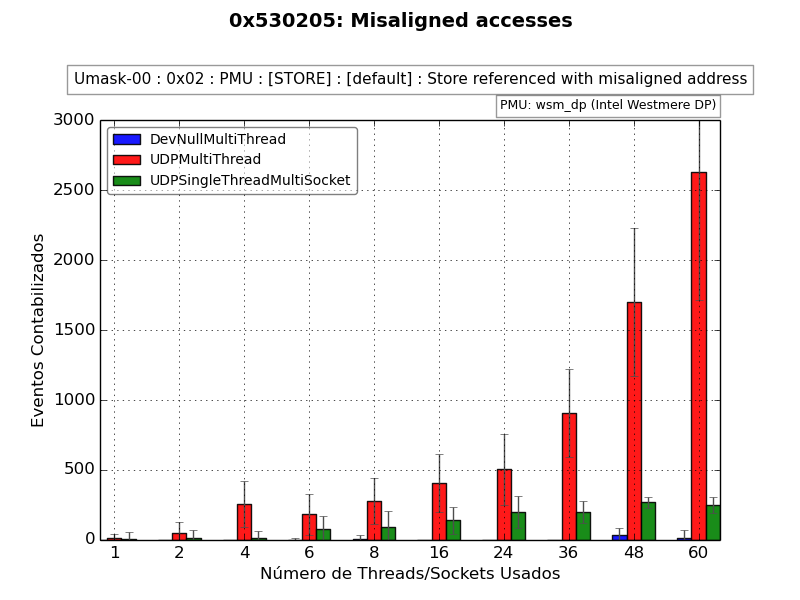
\includegraphics[width=.47\textwidth]{resultados/pcounters/r530205.png}
	\label{fig:pcounterLLCf}
}
\caption{Resultados asociados al comportamiento del último nivel de caché y memoria principal.}
\label{fig:pcounterLLC}
\end{figure}


\begin{figure}[ph!]
\centering
\subfigure[]{
	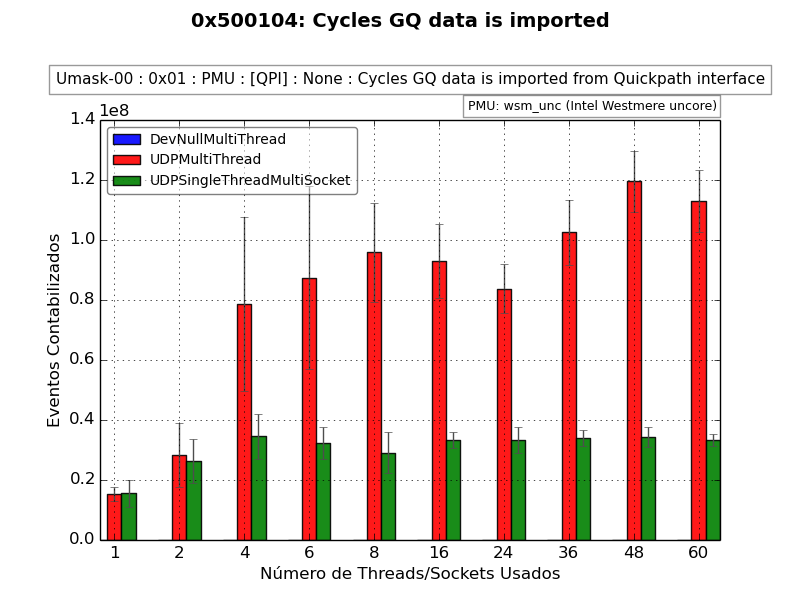
\includegraphics[width=.47\textwidth]{resultados/pcounters/r500104.png}
	\label{fig:pcounterQPIa}
}
\subfigure[]{
	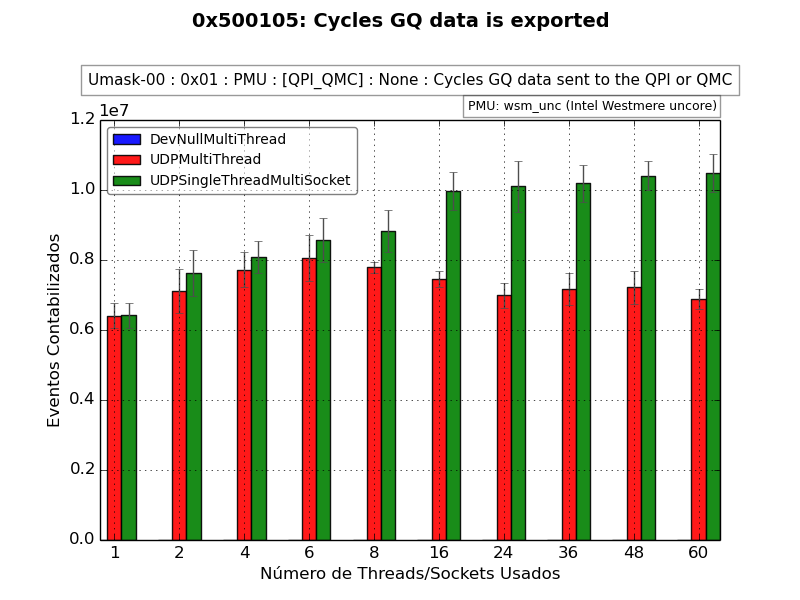
\includegraphics[width=.47\textwidth]{resultados/pcounters/r500105.png}
	\label{fig:pcounterQPIb}
}
\subfigure[]{
	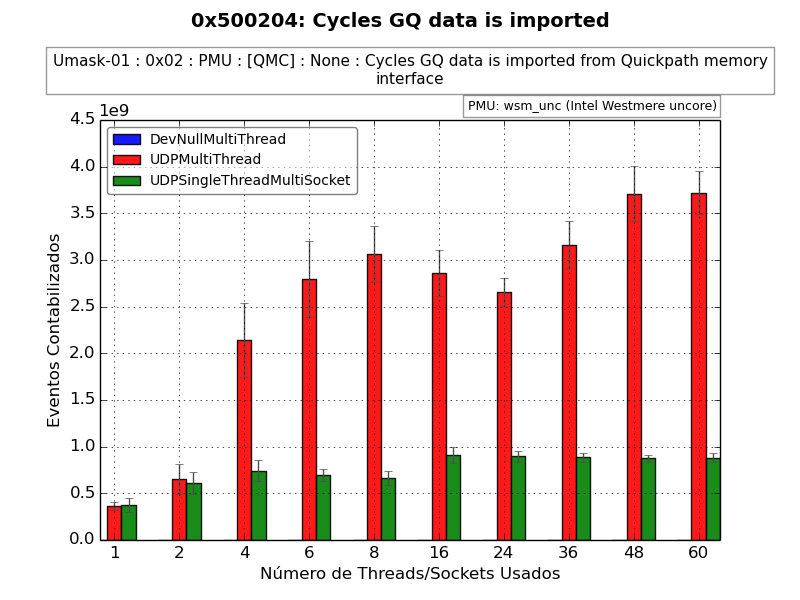
\includegraphics[width=.47\textwidth]{resultados/pcounters/r500204.png}
	\label{fig:pcounterQPIc}
}
\subfigure[]{
	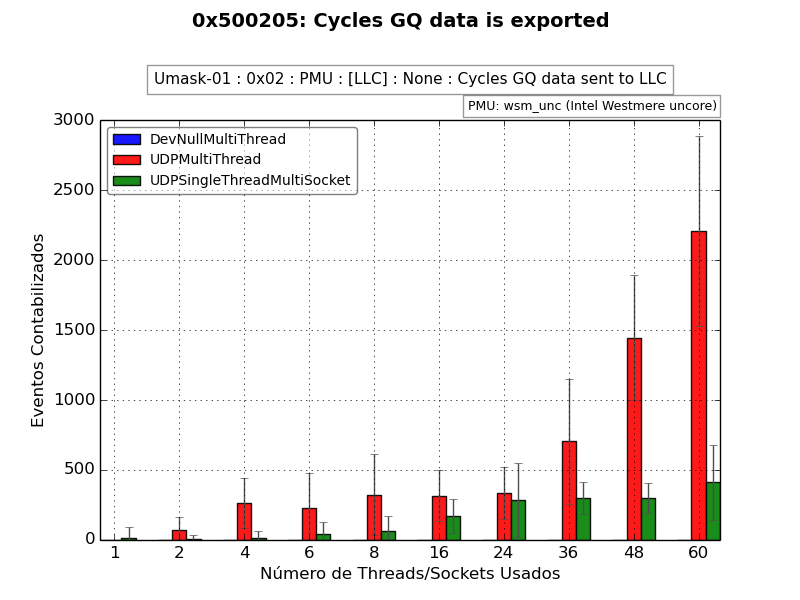
\includegraphics[width=.47\textwidth]{resultados/pcounters/r500205.png}
	\label{fig:pcounterQPId}
}
\subfigure[]{
	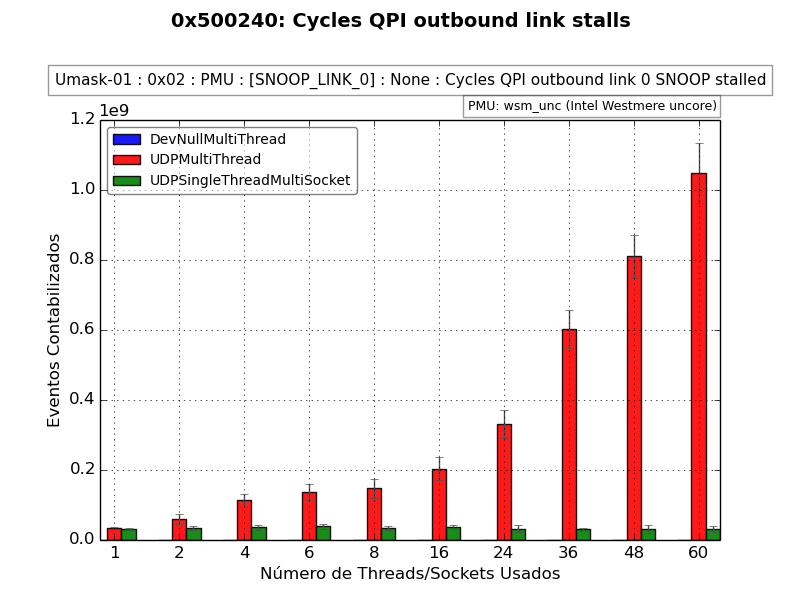
\includegraphics[width=.47\textwidth]{resultados/pcounters/r500240.png}
	\label{fig:pcounterQPIe}
}
\caption{Resultados asociados al comportamiento los canales y estructuras de comunicación del Intel® \emph{QuickPath}.}
\label{fig:pcounterQPI}
\end{figure}


\begin{figure}[ph!]
\centering
\subfigure[]{
	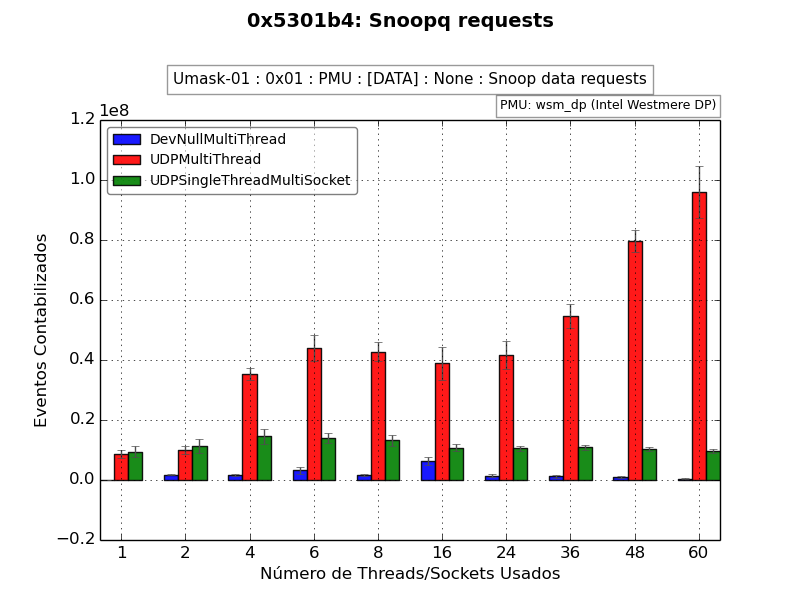
\includegraphics[width=.47\textwidth]{resultados/pcounters/r5301b4.png}
	\label{fig:pcounterSNOOPa}
}
\subfigure[]{
	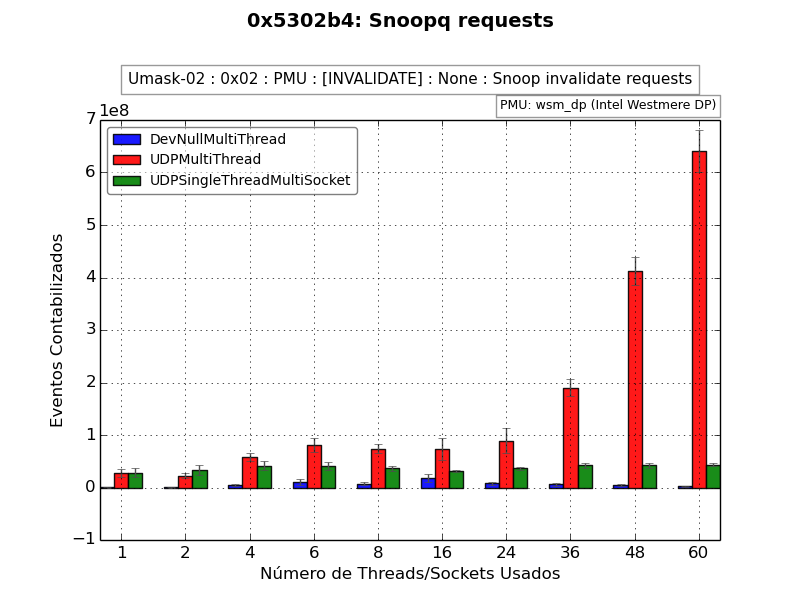
\includegraphics[width=.47\textwidth]{resultados/pcounters/r5302b4.png}
	\label{fig:pcounterSNOOPb}
}
\subfigure[]{
	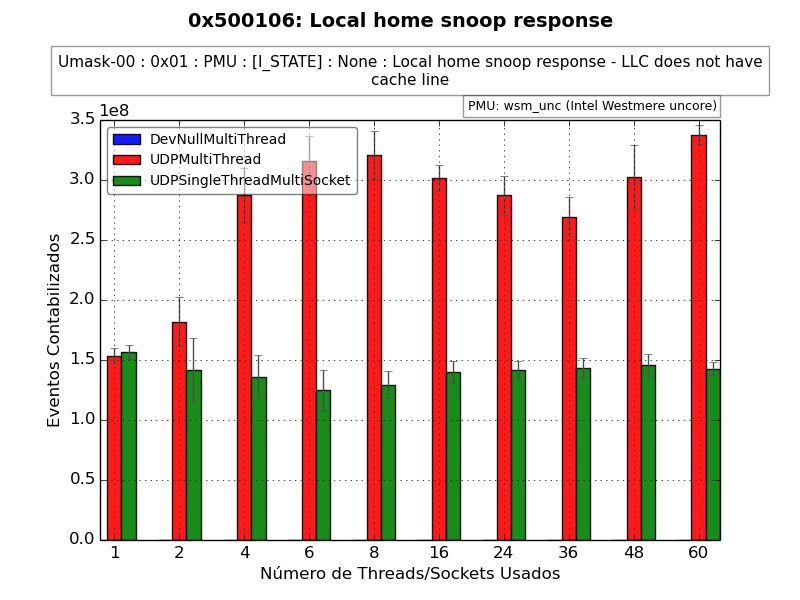
\includegraphics[width=.47\textwidth]{resultados/pcounters/r500106.png}
	\label{fig:pcounterSNOOPc}
}
\subfigure[]{
	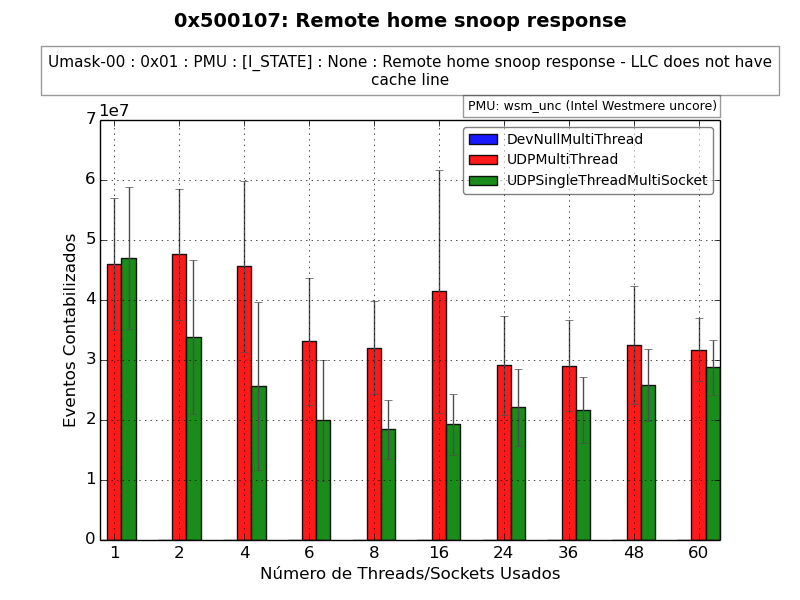
\includegraphics[width=.47\textwidth]{resultados/pcounters/r500107.png}
	\label{fig:pcounterSNOOPd}
}
\subfigure[]{
	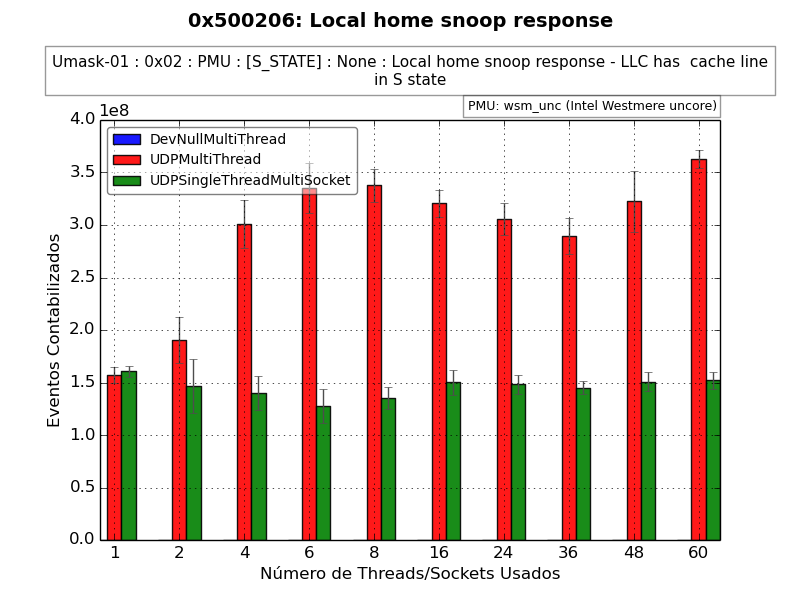
\includegraphics[width=.47\textwidth]{resultados/pcounters/r500206.png}
	\label{fig:pcounterSNOOPe}
}
\caption{Resultados asociados al comportamiento del mecanísmo de control \emph{SNOOP}.}
\label{fig:pcounterSNOOP}
\end{figure}

\section{Análisis y Discusión de Resultados}

Los diferentes resultados presentados en la sección anterior comparten una serie de características comunes importantes de resaltar: En primer lugar, la experimentación sobre el dispositivo virtual \verb=dev_null= presentó prácticamente un nulo registro a nivel de los eventos contabilizados. Una situación esperable pues como se adelantó al momento de diseñar el experimento, éste dispositivo fue elegido como parte de la prueba por ser un dispositivo virtual libre de protecciones ante concurrencia, de manera que su registro da pistas de la correcta activación de las labores de registro de eventos.

Otro rasgo general interesante es que los comportamientos entre el caso \emph{UDPMultiThread} y \emph{UDPSingleThreadMultiSocket} presentan notables diferencia en prácticamente todos los eventos inspeccionados en el caso de estudio, lo cual, más allá de los distintos valores registrados, corrobora que existe una significativa diferencia entre los dos enfoques de consumo de datos (compartición del socket con múltiples hilos contra consumo exclusivo de socket).

En las secciones siguientes se analizan en detalle cada uno de los grupos de resultados rescatados en ésta prueba.

\subsection{Comportamiento de caché de datos de nivel 1}
Los resultados registrados con respecto al comportamiento del caché de datos de nivel 1 (Ver figura \ref{fig:pcounterL1}) evidencian un claro comportamiento desigual entre los escenarios de consumo concurrente vs. consumo exclusivo. Como se aprecia en la mayoría de los resultados de dicha prueba, las tendencias entre ambos escenarios son similares hasta la aplicación de dos hilos, pero al incorporar más hilos de ejecución rápidamente los registros de eventos contabilizados se disparan en el caso multi-hilo, evidenciando una mayor actividad a nivel de caché de datos de nivel 1.

Otro dato interesante a resaltar es el fenómeno de \emph{caché bouncing} expresado en éste resultado. Cómo se puede apreciar, los resultados de las figuras \ref{fig:pcounterL1b}) y \ref{fig:pcounterL1c}) que expresan la cantidad de líneas de caché en estado modificado (de acuerdo a la nomenclatura \emph{MESI}) aumentan progresivamente a medida que se incrementan los hilos consumiendo datos del socket compartido, apoyando la idea de que el escenario concurrente contribuye a una mayor sobre corrección de líneas de caché, lo que puede contribuir en una degradación de la performance del sistema. Lo anterior es nuevamente avalado por el resultado de la figura \ref{fig:pcounterL1d}), que ilustra la acción de los protocolos de corrección y coordinación para modificar estados de líneas de caché. Vale decir, éste resultado muestra cómo los mecanismos de coordinación del sistema están operando desde componentes ajenas a cada Core para corregir líneas que han sido modificadas en otro procesador, otro indicio de que la modificación concurrente de una estructura compartida termina impactando al sistema completo.

Una última reflexión de éste resultado da cuenta de cómo las tendencias crecientes registradas por los eventos relacionados al caché de datos de nivel 1 se ajustan a la registrada por los tiempos prácticos de ejecución del caso de estudio, dando espacio para entender una correlación entre ambos fenómenos.

\subsection{Comportamiento de protocolo MESIF}
En el caso del protocolo MESIF, los resultados registrados a lo largo del caso de estudio (Ver figura \ref{fig:pcounterMESIF})) dan cuenta de dos situaciones a destacar relacionadas a los eventos detectados por concepto de escrituras de líneas de caché de nivel 1 a nivel 2, fenómeno que indica que un valor presente en ambos niveles de caché sufrió una modificación que hace que se propague hacia los niveles de caché inferiores.
La figura \ref{fig:pcounterMESIFa}) presenta el total de sobre escrituras realizadas desde el caché de datos de nivel 1 al caché de nivel 2. Es fácil notar que las tendencias dominantes nuevamente se atribuyen al escenario multi-hilo, que sobrepasa ampliamente al caso de lectura exclusiva desde un socket. Ésta situación respalda el escenario descrito en el análisis previo sobre el comportamiento de caché de datos de nivel 1, donde las sobre correcciones ocurridas en el sistema producto de la modificación de un recurso compartido termina aumentando excesivamente la comunicación práctica entre componentes. En el caso del resultado de la figura \ref{fig:pcounterMESIFb}) la situación resulta aún más dramática. 

En ese resultado se contabilizan los eventos de sobre escritura desde nivel 1 a nivel 2 sobre líneas que presentan estado \emph{Invalid} de acuerdo al protocolo \emph{MESI}, es decir, corrección de valores que ya fueron descartados por otro componente del sistema. Ésta situación da cuenta de cómo la coordinación a nivel de las líneas de caché se va tornando caótica a medida que se intensifican los escenarios concurrentes en el acceso al socket. Cabe destacar que tal como antes, las tendencias generales de los eventos registrados en el caso concurrente se adecúan mucho con la del tiempo del caso de estudio.

\subsection{Comportamiento de Predicción de ejecución del Procesador}
Una de las características fundamentales de los equipos modernos es la capacidad de anticipación de ciertas operaciones a realizar, ya sea cómputo de ciertos valores así como modificaciones o accesos a porciones de memoria. Para ello, durante la ejecución de un programa en que pueden continuar distintas secuencias de pasos, el sistema pre calcula el valor de algunos flujos a seguir de manera de anticiparse a dicho momento. Sin embargo, existen situaciones en que tal predicción resulta errónea con el costo de, primero, descartar los datos computados y, segundo, recalcular los valores necesarios. Tal escenario es denominado \emph{Branch Misprediction} y es justamente lo retratado por los resultados de la figura \ref{fig:pcounterMissBranchPrediction}).

Como se aprecia en los resultados, la cantidad de predicciones erróneas del sistema se dispara a medida que se incorporan hilos en el consumo de datos, escenario que necesariamente termina impactando los tiempos de operación y procesamiento finales. Siguiendo la tendencia de los valores recopilados por concepto de eventos muestreados, tanto los resultados de las figuras \ref{fig:pcounterMissBranchPredictiona}) como \ref{fig:pcounterMissBranchPredictionb}) siguen la misma tendencia de los tiempos finales, contribuyendo evidenciando más pistas de que la compartición del Internet socket termina degenerando el sistema.

\subsection{Comportamiento de fallo en solicitud de datos}
El resultado de la figura \ref{fig:pcounterOFFCore} refleja la dinámica de llamadas que realizan las distintas CPU solicitando datos que no disponen en sus bancos de memoria directos. Nuevamente el caso al usar múltiples hilos domina ampliamente sobre el escenario de lectura exclusiva.

El resultado de la figura \ref{fig:pcounterOFFCorea} ilustra el registro de solicitudes para leer datos en porciones ajenas al núcleo en cuestión. Es particularmente interesante que la tendencia frente al caso concurrente es muy similar al comportamiento detectado en el estudio de porcentajes de llamadas a funciones de bloqueo, abriendo la posibilidad de que dicha similitud se deba a que como el spinlock de protección del socket compartido sea una referencia cruzada entre todos los threads, su localización exacta varíe de momento en momento, haciendo necesario éste tipo de comunicación para dicha validación.

\subsection{Comportamiento de caché de nivel 2}
Similar al caso de los registros de caché de datos de nivel 1, el nivel 2 (Ver figura \ref{fig:pcounterL2}) presenta una dinámica de modificación que se acrecienta a medida que se incorporan más threads, siguiendo lo que ha sido la tónica de los demás resultados.

Un resultado particularmente interesante es el registrado en la figura \ref{fig:pcounterL2b} y \ref{fig:pcounterL2e} que hacen referencia a modificaciones en caché de nivel 2 de tipo \emph{RFO (Request For Ownership)}. Según dicta el protocolo MESI, una línea de caché sólo puede ser escrita si presenta un estado \textbf{M - Modificada} o \textbf{E - Exclusiva}. En caso de presentar un estado \textbf{S - Compartida} las copias deben ser invalidadas antes de la modificación, acción que se realiza por medio de las solicitudes \emph{RFO}. En éste resultado, se aprecia como claramente, las solicitudes de dicho tipo para modificación de líneas de caché en segundo nivel se desata frente al aumento de hilos consumiendo el mismo socket. Más evidencia para entender que, al tener un recurso compartido en distintas porciones del sistema, las modificaciones sobre el mismo se vuelven más significativas y perjudiciales al sistema completo.

\subsection{Comportamiento del último nivel de caché}
La dinámica del último nivel de memoria resulta la menos significativa en términos del impacto para con el caso de estudio, dado que es más inusual que se lleven a éste nivel las referencias que se postulan responsables del fenómeno estudiado. Sin embargo, los resultados de éste estudio presentes en la figura \ref{fig:pcounterLLC}) no dejan de ser interesantes.

Como ha sido tendencia en todos los resultados presentados, la compartición del socket entre diferentes hilos también impacta las referencias alocadas en éste nivel de datos, aunque sin seguir exactamente las mismas tendencias reconocidas a lo largo del estudio. Aun así, éstos resultados son importantes pues en éste nivel de memoria, la latencia en el acceso a los datos es la más significativa, lo que hace que un alto tráfico de la misma impacte en los tiempos finales también del caso de estudio.

\subsection{Comportamiento de los canales de comunicación propios de la arquitectura Intel® \emph{QuickPath}}

Los resultados de la figura \ref{fig:pcounterQPI} dan cuenta del nivel de comunicación de salida y entrada sobre los distintos nodos NUMA del sistema. En éste resultado se reconocen 3 tendencias principales:
\begin{itemize}
\item Figuras \ref{fig:pcounterQPIa} y \ref{fig:pcounterQPIc} que ilustran la cantidad de ocurrencias de importación de información, vale decir, el arribo de datos desde alguna porción externa al núcleo de procesamiento. En éste caso, las tendencias son similares a lo que ha marcado la tendencia general de los demás resultados, presentando una amplia dominación de los valores del caso concurrente.
\item Figura \ref{fig:pcounterQPIb}, que da cuenta de los niveles ce comunicación producidos por concepto de exportación de datos por los canales \emph{QuickPath} a otro nodo NUMA o a los bancos de memoria. En éste caso las tendencias son similares para los casos de acceso concurrente y para el acceso exclusivo hasta los 6 hilos de consumo. En escenarios de mayor concurrencia, el caso multi-hilo prosigue su aumento de eventos de exportación de datos mientras en el caso de accesos exclusivos, se comienzan a reducir. La tendencia en éste caso se repite con respecto a una curva de naturaleza logarítmica que se adecúa a los tiempos netos conseguidos en el caso de estudio.
\item Figuras \ref{fig:pcounterQPId} y \ref{fig:pcounterQPIe}. La primera ilustra la salida o exportación de datos desde el núcleo de procesamiento al último nivel de caché. La segunda se refiere al número de ciclos de procesamiento en que los canales QPI se estancan debido a falta de crédito en los protocolos de nivel de la capa Link de la arquitectura \emph{QuickPath}. Ambos con crecimientos muy significativos a medida que se incrementa el número de hilos y que se separan rápidamente de los registros en el escenario de acceso exclusivo al socket. Se debe prestar especial atención al resultado de la figura \ref{fig:pcounterQPIe} correspondiente a los ciclos de estancamiento pues, dicha situación da cuenta de que la interacción en los canales de comunicación está siendo tan intensa que está saturando los mismos, complicando la transmisión efectiva de datos a nivel de los canales de comunicación y cayendo en los denominados “ciclos muertos” por los mismos protocolos definidos para coordinar la comunicación en ésta arquitectura. Vale decir, es un síntoma de alta comunicación por los canales QPI.
\end{itemize}
En términos generales, los resultados de ésta sección siguen avalando el diagnóstico original de \emph{caché bouncing} por compartición del socket.

\subsection{Comportamiento de mecanismos de control del protocolo \emph{SNOOP}}
El último apartado de resultados presentado en la figura \ref{fig:pcounterSNOOP} corresponde a la interacción dada por los mecanismos de coordinación de caché del protocolo \emph{SNOOP}. A pesar de que en todos los escenarios, los registros de la prueba multi-hilo dominan por sobre los registrados en la prueba de acceso exclusivo, se visualizan dos comportamientos principalmente.

Los resultados de las figuras \ref{fig:pcounterSNOOPc}, \ref{fig:pcounterSNOOPd} y \ref{fig:pcounterSNOOPe} dan cuenta del uso de mecanismos de SNOOP para correcciones al último nivel de acuerdo a los cambios de estado del protocolo MESI. En éste caso, las tendencias son más variadas pero se preserva la situación de mando del caso multi-hilo en todos los resultados. Finalmente, los resultados de las figuras \ref{fig:pcounterSNOOPa} y \ref{fig:pcounterSNOOPb} dan cuenta de la cantidad de mensajes de solicitud de datos de líneas de caché o de marcación de invalidez de líneas de caché de niveles primario o secundario. Ambas tendencias son de crecimiento acelerado y de basto dominio en el caso concurrente. Nuevamente ésta situación avala el diagnóstico de \emph{caché bouncing} en el caso multithread.

\subsection{Correlación de Eventos}
Para poder comprender mejor la tendencia de comportamiento en el experimento entre los distintos eventos capturados se repasaron posibles mecanismos de visualziación que permitieran una simple comparación entre dichas mediciones. Se optó por emplear una visualziación mediante el uso de una matriz de correlación\footnote{\url{https://en.wikipedia.org/wiki/Correlation_and_dependence#Correlation_matrices}}, de manera de poder detectar facilmente conjuntos de eventos relacionados, ello combinando algúna estratégia de clusterización en el proceso de visualizar los datos. Ésta técnica es muy práctica y se ha empleado en otros escenarios sobre el mismo kernel en otras investigaciones con buenos resultados \cite{paper:clusteringKernel}.

Los eventos sobre los que se prestan especial atención son los relacionados a los criterios de selección antes explícitos, agrupados en la tabla \ref{table:eventos}, y cuya traducción a códigos de registro viene dada por la tabla \ref{table:codigoseventos}.

\begin{table}[]
\centering
\begin{tabular}{|l|l|p{0.58\linewidth}|}
\hline
Nivel de Inspección                 & Registro & Descripción                                                \\ \hline
\multirow{8}{*}{Uso de QPI}         & r500104  & Cycles GQ data is imported from Quickpath interface        \\ \cline{2-3} 
                                    & r500204  & Cycles GQ data is imported from Quickpath memory interface \\ \cline{2-3} 
                                    & r500404  & Cycles GQ data is imported from LLC                        \\ \cline{2-3} 
                                    & r500105  & Cycles GQ data sent to the QPI or QMC                      \\ \cline{2-3} 
                                    & r500205  & Cycles GQ data sent to LLC                                 \\ \cline{2-3} 
                                    & r500405  & Cycles GQ data sent to cores                               \\ \cline{2-3} 
                                    & r500420  & Quickpath Home Logic remote read requests                  \\ \cline{2-3} 
                                    & r500820  & Quickpath Home Logic remote write requests                 \\ \hline
\multirow{3}{*}{Snoop}              & r530451  & L1D cache lines replaced in M state                        \\ \cline{2-3} 
                                    & r530251  & L1D cache lines allocated in the M state                   \\ \cline{2-3} 
                                    & r530851  & L1D snoop eviction of cache lines in M state               \\ \hline
\multirow{15}{*}{Pasos entre Cache} & r500108  & Number of LLC read hits                                    \\ \cline{2-3} 
                                    & r500208  & Number of LLC write hits                                   \\ \cline{2-3} 
                                    & r500109  & Number of LLC read misses                                  \\ \cline{2-3} 
                                    & r500209  & Number of LLC write misses                                 \\ \cline{2-3} 
                                    & r50010a  & LLC lines allocated in M state                             \\ \cline{2-3} 
                                    & r50020a  & LLC lines allocated in E state                             \\ \cline{2-3} 
                                    & r50040a  & LLC lines allocated in S state                             \\ \cline{2-3} 
                                    & r50080a  & LLC lines allocated in F state                             \\ \cline{2-3} 
                                    & r500f0a  & LLC lines allocated                                        \\ \cline{2-3} 
                                    & r50010b  & LLC lines victimized in M state                            \\ \cline{2-3} 
                                    & r50020b  & LLC lines victimized in E state                            \\ \cline{2-3} 
                                    & r50040b  & LLC lines victimized in S state                            \\ \cline{2-3} 
                                    & r50080b  & LLC lines victimized in I state                            \\ \cline{2-3} 
                                    & r50100b  & LLC lines victimized in F state                            \\ \cline{2-3} 
                                    & r501f0b  & LLC lines victimized                                       \\ \hline
\multirow{4}{*}{MESI}               & r501f0b  & L2 data demand loads in E state                            \\ \cline{2-3} 
                                    & r530126  & L2 data demand loads in I state (misses)                   \\ \cline{2-3} 
                                    & r530326  & L2 data demand loads in M state                            \\ \cline{2-3} 
                                    & r530526  & L2 data demand loads in S state                            \\ \hline
\end{tabular}
\caption{Colección de eventos resumidos para la inspección de los canales de comunicación del sistema en escenarios multithread.}
\label{table:codigoseventos}
\end{table}

\begin{figure}[h!]
	\centering
	\hspace*{\fill}
	\subfigure[]{
		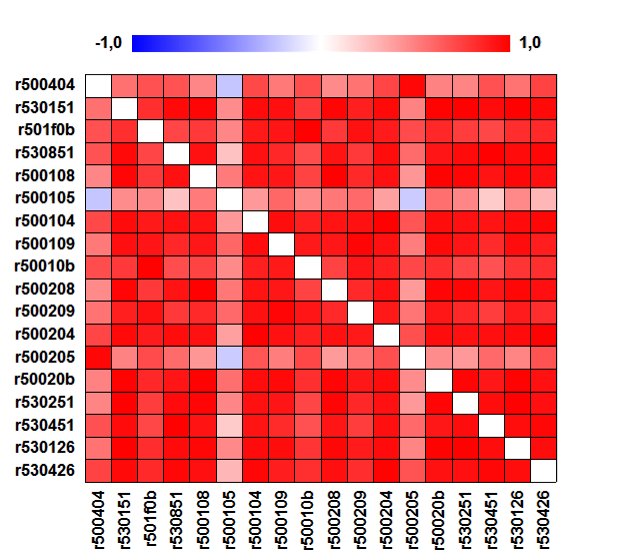
\includegraphics[width=.45\textwidth]{imagenes/corrgram0.png}
		\label{fig:corrgram:a}
	}\hfill
	\subfigure[]{
		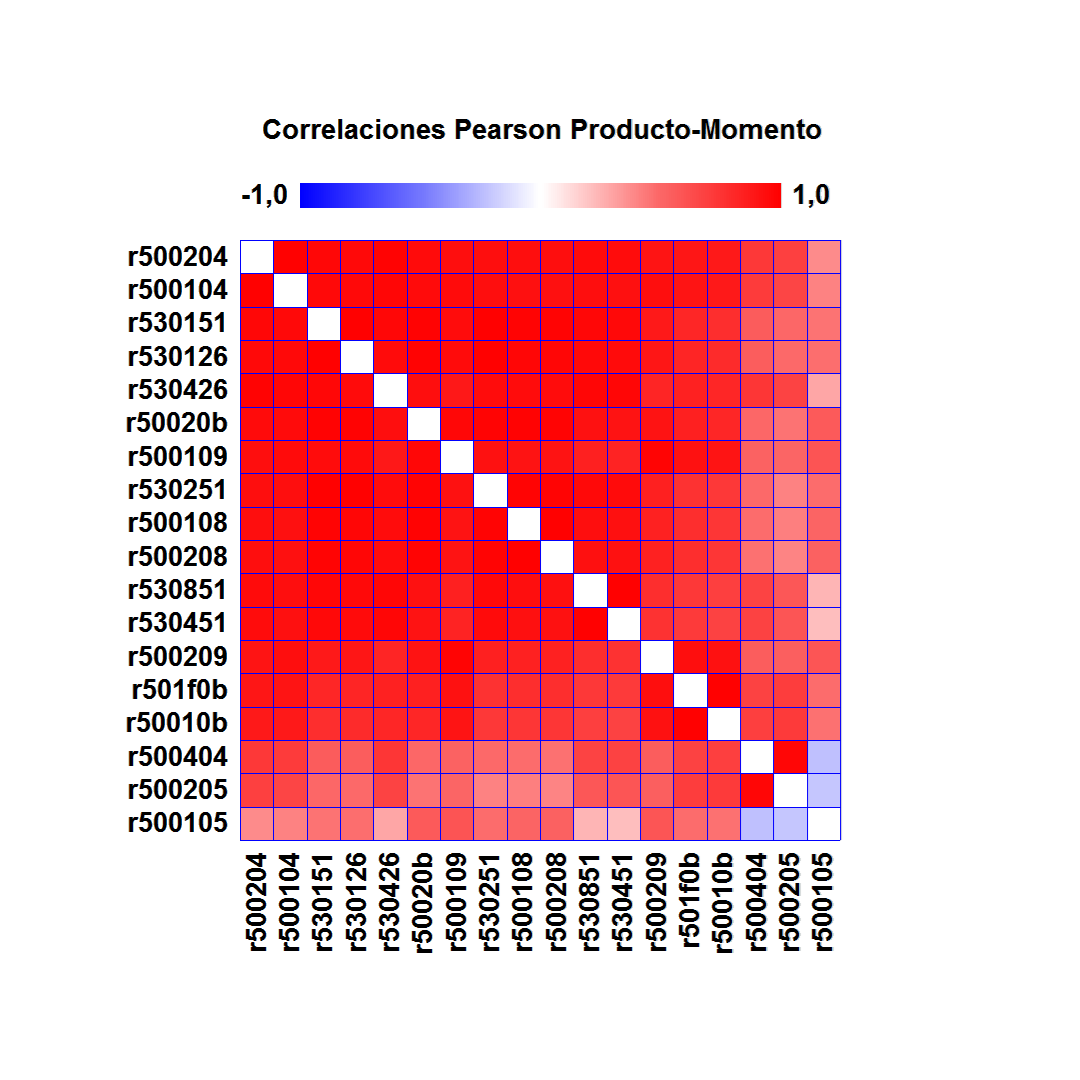
\includegraphics[width=.45\textwidth]{imagenes/corrgram1.png}
		\label{fig:corrgram:b}
	}
	\caption{Resultado de la visualización de la matriz de correlación con el software \emph{statgraphics}. En la figura \ref{fig:corrgram:a} se pueden visualizar los datos en bruto, mientras en \ref{fig:corrgram:b} se presentan los datos agrupados, tras ordenar la matriz de acuerdo al criterio de los vectores propios, logrando un efecto clusterizador.}
	\label{fig:corrmatrix}
	\hspace*{\fill}
\end{figure}


Para ésta tarea, se empleó el software de visualización \emph{statgraphics}\footnote{\url{http://www.statgraphics.com/}}. El software tiene la capacidad de generar una visualización aprovechando un ordenamiento por medio del primer vector propio de la matriz de correlación construida, de manera de generar un efecto clusterizador sobre los datos, agrupando aquellos con alta correlación.

Como se puede apreciar en su resultado, la mayoría de los eventos estudiados en la matriz de correlación presentan un enorme grado de similitud en sus tendencias (Próximos a 1), lo que combinado con los resultados anteriores de las curvas de registro colectadas con el estudio de \emph{performance counters} da que el grueso de los registros de eventos colectados sigue la misma tendencia de crecimiento del tiempo registrado por el caso de estudio, lo que contribuye nueva evidencia de que el conjunto de mecanismos de comunicación verificables por ésta vía está comprometida por efecto del acceso concurrente a una estructura única.

\section{Conclusiones}
A raíz del estudio de canales de comunicación de hardware del sistema se pueden rescatar varios aspectos interesantes:
\begin{itemize}
\item Se identificó un comportamiento creciente en el registro de eventos capturados, trasversal entre todos los eventos postulados en el estudio.
\item Se recabó evidencia de distintos niveles de comunicación cómo transferencia de valores entre niveles de caché y memoria, en conjunto con la actividad de los protocolos de coherencia y corrección de líneas de caché que apoya la hipótesis del escenario de \emph{caché bouncing} en el sistema estudiado.
\item se determinó experimentalmente que bajo el régimen de acceso concurrente a un mismo socket, se evidencian más problemas reflejados en el aumento de predicciones erróneas de los procesadores y de grandes aumentos en los canales de comunicación de datos entre componentes de procesamiento, evidencia que respalda la sospecha de la existencia de una estructura (el spinlock del socket) altamente compartida y requerida por los distintos cores, situación que degenera en degradaciones importantes del sistema.
\item Al observar en detalle la mayoría de los eventos, se da cuenta de cómo la tendencia de saturación sigue un régimen similar al de los tiempos generales del caso de estudio.
\item La colección de eventos correlacionados evidenció una tendencia generalizada y uniforme sobre los eventos involucrados, los cuales además de estar fuertemente correlacionados entre sí, siguen la misma tendencia de los tiempos del caso de estudio.
\end{itemize}